%%%%%%%%%%%%%%%%%%%%%%%%%%%%%%%%%%%%%%%%%
% Masters/Doctoral Thesis 
% LaTeX Template
% Version 2.4 (22/11/16)
%
% This template has been downloaded from:
% http://www.LaTeXTemplates.com
%
% Version 2.x major modifications by:
% Vel (vel@latextemplates.com)
%
% This template is based on a template by:
% Steve Gunn (http://users.ecs.soton.ac.uk/srg/softwaretools/document/templates/)
% Sunil Patel (http://www.sunilpatel.co.uk/thesis-template/)
%
% Template license:
% CC BY-NC-SA 3.0 (http://creativecommons.org/licenses/by-nc-sa/3.0/)
%
%%%%%%%%%%%%%%%%%%%%%%%%%%%%%%%%%%%%%%%%%

%----------------------------------------------------------------------------------------
%	FELIX NEWCOMMANDS
%----------------------------------------------------------------------------------------
% equalsign with space
\def\eq{\ensuremath{&\quad=\quad}}
% unit vector
\def\uvec#1{\ensuremath{\hat{\mathbf{e}}_{\textup{#1}}}}
% The number `e'.
\def\eu{\ensuremath{\mathrm{e}}}
% The imaginary unit.
\def\iu{\ensuremath{\mathrm{i}}}
% The differential operator.
\def\du{\ensuremath{\mathrm{d}}}
% kappax0
\def\kap{\ensuremath{\mathrm{\kappa_{\textup{x}0}}}}
% kappay0
\def\kapy{\ensuremath{\mathrm{\kappa_{\textup{y}0}}}}

%----------------------------------------------------------------------------------------
%	PACKAGES AND OTHER DOCUMENT CONFIGURATIONS
%----------------------------------------------------------------------------------------

\documentclass[
10pt, % The default document font size, options: 10pt, 11pt, 12pt
%oneside, % Two side (alternating margins) for binding by default, uncomment to switch to one side
english, % ngerman for German
singlespacing, % Single line spacing, alternatives: onehalfspacing or doublespacing
%draft, % Uncomment to enable draft mode (no pictures, no links, overfull hboxes indicated)
%nolistspacing, % If the document is onehalfspacing or doublespacing, uncomment this to set spacing in lists to single
%liststotoc, % Uncomment to add the list of figures/tables/etc to the table of contents
%toctotoc, % Uncomment to add the main table of contents to the table of contents
%parskip, % Uncomment to add space between paragraphs
%nohyperref, % Uncomment to not load the hyperref package
%headsepline, % Uncomment to get a line under the header
%chapterinoneline, % Uncomment to place the chapter title next to the number on one line
%consistentlayout, % Uncomment to change the layout of the declaration, abstract and acknowledgements pages to match the default layout
]{MastersDoctoralThesis} % The class file specifying the document structure

\usepackage[utf8]{inputenc} % Required for inputting international characters
\usepackage[T1]{fontenc} % Output font encoding for international characters
\usepackage{libertine}
\usepackage[libertine,cmintegrals,cmbraces,vvarbb]{newtxmath}
\usepackage{bookmark} % add contents to bookmarks
\usepackage{listings} % include code
\lstset{
	basicstyle=\footnotesize, % alle listings winzig drucken (meine Standardeinstellung)
	keywordstyle=\color{black}\bfseries, % Schlüsselwörter fett und schwarz drucken
	commentstyle=\color{blue},% Kommentare blau drucken}
	showstringspaces=false} % Strings im Code ohne Kenntlichmachung von Leerzeichen - finde ich angebracht und empfehlenswert

\usepackage[backend=bibtex, style=numeric, natbib=true, isbn=false, backref=true, sorting=none, url=false]{biblatex} % Use the bibtex backend with the authoryear citation style (which resembles APA)
\addbibresource{bibliography.bib} % The filename of the bibliography
\usepackage[autostyle=true]{csquotes} % Required to generate language-dependent quotes in the bibliography

%----------------------------------------------------------------------------------------
%	FELIX PACKAGES
%----------------------------------------------------------------------------------------
%\usepackage{amsmath}
\usepackage{sidecap} % captions beside figure with \begin{SCfigure}
\usepackage[hang]{footmisc}
\usepackage{rotating} % landscape figure
\usepackage{pdflscape}
\urlstyle{same} % url schrift normal
\usepackage[export]{adjustbox} % algin two side by side graphics, for example top align
%\usepackage{flafter} % avoids that figures are floated before they were defined

%----------------------------------------------------------------------------------------
%	MARGIN SETTINGS
%----------------------------------------------------------------------------------------

\geometry{
	paper=a4paper, % Change to letterpaper for US letter
	inner=2.5cm, % Inner margin
	outer=3.8cm, % Outer margin
	bindingoffset=.5cm, % Binding offset
	top=1.5cm, % Top margin
	bottom=1.5cm, % Bottom margin
%	showframe, % Uncomment to show how the type block is set on the page
}
	
%----------------------------------------------------------------------------------------
%	THESIS INFORMATION
%----------------------------------------------------------------------------------------
\newcommand{\ttitle}{Optimization of the BESSY II optics for the VSR project - Increase the installation length for the VSR cryomodule in the T2 section of the BESSY~II storage ring} % Your thesis title, this is used in the title and abstract, print it elsewhere with \ttitle
\supervisor{Prof. Dr. Andreas \textsc{Jankowiak}\\Dr. Paul \textsc{Goslawski}} % Your supervisor's name, this is used in the title page, print it elsewhere with \supname
\examiner{} % Your examiner's name, this is not currently used anywhere in the template, print it elsewhere with \examname
\degree{ Bachelor of Science (B. Sc.)} % Your degree name, this is used in the title page and abstract, print it elsewhere with \degreename
\author{Felix \textsc{Andreas}} % Your name, this is used in the title page and abstract, print it elsewhere with \authorname
\addresses{} % Your address, this is not currently used anywhere in the template, print it elsewhere with \addressname

\subject{Physics} % Your subject area, this is not currently used anywhere in the template, print it elsewhere with \subjectname
\keywords{Physics} % Keywords for your thesis, this is not currently used anywhere in the template, print it elsewhere with \keywordnames
\university{\href{http://hu-berlin.de}{Humboldt-Universität zu Berlin}} % Your university's name and URL, this is used in the title page and abstract, print it elsewhere with \univname
\department{\href{https://www.physik.hu-berlin.de/en/department}{Department of Physics}} % Your department's name and URL, this is used in the title page and abstract, print it elsewhere with \deptname
\group{\href{http://www.helmholtz-berlin.de/forschung/oe/fg/beschleunigerphysik/}{Institute for Accelerator Physics}} % Your research group's name and URL, this is used in the title page, print it elsewhere with \groupname
\faculty{\href{https://www.hu-berlin.de/en/institutions/faculties-and-departments/mathematics-natural-sciences}{Faculty of Mathematics and Natural Sciences}} % Your faculty's name and URL, this is used in the title page and abstract, print it elsewhere with \facname

\AtBeginDocument{
\hypersetup{pdftitle=\ttitle} % Set the PDF's title to your title
\hypersetup{pdfauthor=\authorname} % Set the PDF's author to your name
\hypersetup{pdfkeywords=\keywordnames} % Set the PDF's keywords to your keywords
}

\begin{document}

\frontmatter % Use roman page numbering style (i, ii, iii, iv...) for the pre-content pages

\pagestyle{plain} % Default to the plain heading style until the thesis style is called for the body content

%----------------------------------------------------------------------------------------
%	TITLE PAGE
%----------------------------------------------------------------------------------------

\newgeometry{hmarginratio=1:1} %seite nicht einrücken
\begin{titlepage}
	\pdfbookmark{Title page}{Title page}
	\begin{center}
		\begin{figure}
\includegraphics[width = \linewidth]{images/hulogo/hukombi_bbw_op}\end{figure}
		\vspace*{.06\textheight}
		%{\scshape\LARGE \univname\par}\vspace{1.5cm} % University name
		\textsc{\Large Bachelor Thesis}\\[0.5cm] % Thesis type

		%\HRule \\[0.4cm] % Horizontal line
		\vspace{0.4cm}{\Large \bfseries \ttitle\par}\vspace{0.4cm}\vspace{1.5cm} % Thesis title
		%\HRule \\[1.5cm] % Horizontal line

		\begin{minipage}[t]{0.42\textwidth}
			\begin{flushleft} \large
				\emph{Author:}\\
				\href{felix.andreas@physik.hu-berlin.de}{\authorname} % Author name - remove the \href bracket to remove the link
			\end{flushleft}
		\end{minipage}
		\begin{minipage}[t]{0.42\textwidth}
			\begin{flushright} \large
				\emph{Supervisor:} \\
				\href{http://}{\supname} % Supervisor name - remove the \href bracket to remove the link  
			\end{flushright}
		\end{minipage}\\[2cm]

		\vfill

		\large \textit{A thesis submitted in fulfillment of the requirements\\ for the degree of \degreename}\\[0.3cm] % University requirement text
		\textit{in the}\\[0.4cm]
		\facname\\\deptname\\[2cm] % Research group name and department name

		\vfill

		{\large \today}\\[4cm] % Date
		%\includegraphics{width = 0.3\linewidth]{images/hulogo/husiegel_bw} % University/department logo - uncomment to place it

		\vfill
	\end{center}
\end{titlepage}
\restoregeometry

%----------------------------------------------------------------------------------------
%	ABSTRACT PAGE
%----------------------------------------------------------------------------------------

\begin{abstract}
	\addchaptertocentry{\abstractname} % Add the abstract to the table of contents
	BESSY\,II is a third generation synchrotron light source located in Berlin Adlershof. It purpose is to provide extremely brilliant synchrotron light pulses in the range from long terahertz radiation to hard X-rays. In the last several years, there is a continuously increasing interest in the short pulse operation. Therefore the next major upgrade is to enable a storage ring with short and long pulses, simultaneously. This variable pulse-length storage ring can be achieved due to the installation of additional superconducting high gradient cavities. The cavities will be assembled into one cryomodule in the T2 section of the storage ring. As this module needs more space then initially assumed, the idea is to remove two quadrupoles to gain installation length. Linear beam optics computations with an optimization method were used to switch off the quadrupoles in simulations. The different theoretical optics obtained were transfered to the storage ring. For the best solution it was possible to store high current with reasonable injection efficiency and lifetime. The proposed optics of this thesis has to be further optimized in regards to non-linear beam dynamics, but has shown that an enlargement of the installation length is possible.
\end{abstract}


%----------------------------------------------------------------------------------------
%	ABSTRACT PAGE
%----------------------------------------------------------------------------------------
\begin{otherlanguage}{ngerman}
	\begin{abstract}
		%\addchaptertocentry{\abstractname} % Add the abstract to the table of contents
		BESSY\,II ist eine Synchrotronstrahlungsquelle der dritten Generation am Standort Adlershof, welche extrem brilliante Synchrotronpulse im Bereich von langer Terahertzstrahlung bis hin zur harter Röntgenstrahlung erzeugt. Seit mehreren Jahren gibt es ein kontinuierlich zunehmendes Interesse am Betrieb mit ultrakurzen Pulsen. Daher soll mit dem nächsten großen Upgrade die gleichzeitige Erzeugung von kurzen und langen Pulse im Speicherring ermöglicht werden. Dieser Variable Pulslängen-Speicherring kann durch den Einbau zusätzlicher stark fokussierender supraleitender Kavitäten realisiert werden. Diese Kavitäten werden in ein Kryomodul in der T2 Geraden des Speicherringes eingebaut. Da dieses Modul mehr Platz braucht als zunächst angenommen, ist die Idee, zwei Quadrupole auszubauen, um an Einbaulänge zu gewinnen. Mithilfe von linearer Strahloptik und einer Optimierungsmethode wurden die Quadrupole in Simulationen ausgeschaltet. Anschließend wurden die verschiedenen theoretischen Optiken am Speicherring getested. Die beste Lösung ermöglichte das Speichern eines hohen Strom mit guter Injektionseffizienz und Lebensdauer. Die vorgeschlagene Optik dieser Arbeit muss in Bezug auf nichtlineare Strahldynamik weiter optimiert werden, zeigt aber, dass eine Vergrößerung der Einbaulänge möglich ist.
	\end{abstract}
\end{otherlanguage}


%----------------------------------------------------------------------------------------
%	ACKNOWLEDGEMENTS
%----------------------------------------------------------------------------------------

\begin{acknowledgements}
	\addchaptertocentry{\acknowledgementname} % Add the acknowledgements to the table of contents
	An erster Stelle möchte ich mich bei Herrn Professor Andreas Jankowiak bedanken, dass er mir ermöglicht hat, diese Arbeit am Helmholtz-Zentrum Berlin durchzuführen und dass er selbige begutachtet.\\

	\noindent Mein größter Dank geht an Dr. Paul Goslawski, der mich mit viel Engagement richtungsweisend bei meiner Arbeit begleitet hat. Vielen Dank für die Einführung in die Arbeitsgruppe, für zahlreiche Anmerkungen und Kommentare, für deine Ausdauer bei den langen nächtlichen Experimenten und vor Allem für die vielen spannenden physikalischen Diskussionen.\\

	\noindent Ich möchte mich bei Felix Kramer bedanken, der mir bei der Einfindung in die Arbeitsumgebung des Instituts sehr geholfen hat. Danke außerdem für viele Anregungen und Ideen.\\

	\noindent Ich bedanke mich bei meinen Eltern für den motivierenden Beistand und dass sie mir dieses Studium ermöglicht haben.


\end{acknowledgements}

%----------------------------------------------------------------------------------------
%	LIST OF CONTENTS/FIGURES/TABLES PAGES
%----------------------------------------------------------------------------------------
\cleardoublepage
\pdfbookmark[chapter]{\contentsname}{toc}
\tableofcontents % Prints the main table of contents

\cleardoublepage
\pdfbookmark{List of Figures}{List of Figures}
\listoffigures % Prints the list of figures

\cleardoublepage
\pdfbookmark{List of Tables}{List of Tables}
\listoftables % Prints the list of tables

%----------------------------------------------------------------------------------------
%	ABBREVIATIONS
%----------------------------------------------------------------------------------------
\cleardoublepage
\pdfbookmark{Abbreviations}{Abbreviations}
\begin{abbreviations}{ll} % Include a list of abbreviations (a table of two columns)

	\textbf{BESSY} & \textbf{B}erliner \textbf{E}lektronen\textbf{S}peicherring-Gesellschaft für \textbf{SY}nchrotronstrahlung m.b.H.\\\\

	\textbf{BPM} &  \textbf{B}eam \textbf{P}osition \textbf{M}onitor\\\\

	\textbf{DBA} & \textbf{D}ouble \textbf{B}end \textbf{A}chromat\\\\

	\textbf{DOF} & \textbf{D}egree \textbf{O}f \textbf{F}reedom\\\\

	\textbf{ELEGANT} & \textbf{ELE}ctron \textbf{G}eneration \textbf{AN}d \textbf{T}racking\\\\

	% \textbf{ELEMENT} & \textbf{ELE}ctron Bea\textbf{M} \textbf{E}ssentials A\textbf{N}d \textbf{T}racking\\\\

	\textbf{EPICS} & \textbf{E}xperimental \textbf{P}hysics and \textbf{I}ndustrial \textbf{C}ontrol \textbf{S}ystem\\\\

	\textbf{FODO} & A \textbf{F}ocusing n\textbf{O}t focusing  \textbf{D}efocusing n\textbf{O}t focusing magnet structure\\\\

	\textbf{GUI} & \textbf{G}raphical \textbf{U}ser \textbf{I}nterface\\\\

	\textbf{HZB} & \textbf{H}elmholtz-\textbf{Z}entrum \textbf{B}erlin\\\\

	\textbf{ID} & \textbf{I}nsertion \textbf{D}evice\\\\

	\textbf{LOCO} &  \textbf{L}inear \textbf{O}ptics from \textbf{C}losed \textbf{O}rbits\\\\

	\textbf{MML} & \textbf{M}atLab \textbf{M}iddle \textbf{L}ayer\\\\

	\textbf{RF} & \textbf{R}adio \textbf{F}requency\\\\

	\textbf{VSR} & \textbf{V}ariable pulse length \textbf{S}torage \textbf{R}ing\\\\


\end{abbreviations}

%----------------------------------------------------------------------------------------
%	PHYSICAL CONSTANTS/OTHER DEFINITIONS
%----------------------------------------------------------------------------------------

%\begin{constants}{lr@{${}={}$}l} % The list of physical constants is a three column table

% The \SI{}{} command is provided by the siunitx package, see its documentation for instructions on how to use it

%Speed of Light & $c_{0}$ & \SI{2.99792458e8}{\meter\per\second} (exact)\\
%Constant Name & $Symbol$ & $Constant Value$ with units\\

%\end{constants}

%----------------------------------------------------------------------------------------
%	SYMBOLS
%----------------------------------------------------------------------------------------
\cleardoublepage
\pdfbookmark{List of Symbols}{List of Symbols}

\begin{symbols}{lll} % Include a list of Symbols (a three column table)
	%Symbol & Name & Unit \\
	$c$ & Speed of light & \si{\meter\per\second} \\
	$e$ & Elementary charge & \si{\coulomb} \\
	$k$ & Quadrupole strength & \si{\per\square\meter} \\
	$p$ & Momentum & \si{\kilogram\meter\per\second}\\
	$t$ & Time & \si{\second}\\
	$\beta$ & velocity in units of the speed of light & \si{1}\\
	$\gamma$ & Lorentz factor & \si{1}\\
	\addlinespace
	$\textbf{B}$ & Magnetic flux density & \si{\tesla}\\
	$\textbf{E}$ & Electric field & \si{\volt\per\meter}\\
	$\textbf{F}$ & Force & \si{\kilogram\meter\per\square\second}\\
	\addlinespace % Gap to separate the Roman symbols from the Greek
	$\beta_{\textup{x,y}}$ & horizontal, vertical betatron function & \si{\meter} \\
	$\alpha_{\textup{x,y}}$ & horizontal, vertical alpha function & \si{1} \\
	$\gamma_{\textup{x,y}}$ & horizontal, vertical gamma function & \si{\per \meter} \\
	$\epsilon_{\textup{x,y}}$ & horizontal, vertical emittance  & \si{\meter} \\
	$\psi_{\textup{x,y}}$ & horizontal, vertical betatron phase  & \si{1} \\
	$Q_{\textup{x,y}}$ & horizontal, vertical tune & \si{1} \\
	$\eta_{\textup{x,y}}$ & horizontal, vertical dispersion function  & \si{\meter} \\
	$\alpha_\textup{c}$  & Momentum compaction factor & \si{1} \\
	\addlinespace
	$\textbf{X}$ & 6D particle vector & various\\
	$\uvec{x}$ & normal (horizontal) unit vector & \si{\meter}\\
	$\uvec{y}$ & binormal (vertical) unit vector & \si{\meter}\\
	$\uvec{s}$ & tangent unit vector & \si{\meter}\\
	$\uvec{z}$ & unit vector of the particle velocity & \si{\meter}\\
	$x$ & horizontal spatial offset & \si{\meter}\\
	$y$ & vertical spatial offset & \si{\meter}\\
	$s$ & orbit position & \si{\meter}\\
	$z$ & position on the individual particle trajectory & \si{\meter}\\
	$\delta$ & relative momentum deviation& \si{1}\\
	$l$ & longitudinal offset & \si{\meter}\\
	$\rho_{\textup{x0}}, \rho_{\textup{y0}}$ & horizontal, vertical radius of curvature of the orbit& \si{\meter} \\
	$\rho_{\textup{x}}, \rho_{\textup{y}}$ & horizontal, vertical radius of curvature of the particle trajectory& \si{\meter} \\
	$\kappa_{\textup{x0}}, \kappa_{\textup{y0}}$ & horizontal, vertical curvature of the orbit& \si{\per \meter} \\
	$\kappa_{\textup{x}}, \kappa_{\textup{y}}$ & horizontal, vertical curvature of the particle trajectory& \si{\per \meter} \\


\end{symbols}

%%----------------------------------------------------------------------------------------
%%	DEDICATION
%%----------------------------------------------------------------------------------------
%
%\dedicatpdflatex', actual output 'thesory{Dedicated to me, myself and I.} 

%----------------------------------------------------------------------------------------
%	THESIS CONTENT - CHAPTERS
%----------------------------------------------------------------------------------------

\mainmatter % Begin numeric (1,2,3...) page numbering

\pagestyle{thesis} % Return the page headers back to the "thesis" style

% Include the chapters of the thesis as separate files from the Chapters folder
% Uncomment the lines as you write the chapters

\chapter{Introduction} \label{Introduction}
The first section of this chapter introduces the third generation light source BESSY II. The second section gives a brief overview over the Variable Pulse Length Storage Ring project (\textit{VSR}). The challenge of the cavities' installation length is showcased in the third section and is the motivation of this thesis.

\section{BESSY II - A third generation light source}
\begin{figure}
	\centering
	\includegraphics[width = \textwidth]{images/01-BESSY-II-floor-plan.pdf}
	\caption[Floor plan of synchrotron light source BESSY II.]{Floor plan of synchrotron light source BESSY II (extracted from~\cite{Rubrecht_PhD}).}
	\label{fig:Bessy2-plan}
\end{figure}
\begin{table}
	\centering
	\footnotesize
	\caption{Parameters of the BESSY II storage ring.}
	\begin{tabular}{ll}
\toprule
\textbf{Parameter}  &  \textbf{Value}\\
\midrule
nominal energy & 1.7\,GeV\\
circumference & 240\,m\\
RF-frequency & 500\,MHz\\
revolution time & 800\,ns\\
beam current & 300\,mA\\
number of cells & 16\\
number of bending magnets & 32\\
bending radius & 4.361\,m\\
beamlines & $\approx$ 50\\
\bottomrule
\end{tabular}

	\label{tab:mostimportantparameter}
\end{table}

The third generation synchrotron light source BESSY II is located in Berlin Adlershof and is operated by the research institute HZB since 1998. Its purpose is to provide extremely brilliant synchrotron light pulses in the range from long terahertz radiation to hard X-rays. The storage ring has a circumference of 240\,m and is equipped with 50 beamlines. A graphic overview of BESSY II is shown in \autoref{fig:Bessy2-plan}. The most important parameters of the storage ring are listed in \autoref{tab:mostimportantparameter}.

The electrons are emitted by a DC grid cathode and are accelerated up to 90\,keV. In the following linac their energy is increased up to 50\,MeV~\cite{linac}. Next the electrons are transfered to the booster synchrotron, where they are accelerated up to 1.7\,GeV and are than injected to the storage ring cumulatively, so that a beam current of 300\,mA is maintained (\textit{top-up}). The electrons can be saved for up to 10 hours and emit, depending on the type of deflection (bending magnet, wiggler or undulator), photon energies up to 15\,keV.

At BESSY II it is possible to operate the machine in two different modes. Most of the time the storage ring is set to the standard user optics with 15\,ps bunch length. During two weeks of the year the lattice is changed to the low alpha optics, which provide buckets with 3\,ps bunch length~\cite{vsrstudy}. This can be realized by reducing the momentum compaction factor $\alpha_{\textup{c}}$ from  $7 \cdot 10^{-4}$ to $4 \cdot 10^{-5}$. The coherent synchrotron radiation instability leads to a limiting bursting threshold current, which scales with~$\alpha_{\textup{c}}$. Therefore the photon flux has to be reduced significantly in comparison to the standard optics. In this time high flux user are not able to run experiments, which is the reason that the low alpha mode can only be provided for short periods.

%Independent of the optics the 400 available buckets of the storage ring can be filled with different patterns. In the multibunch mode the 300-350 buckets are filled. This allows for a high beam current with high brightness. In the single and few bunch mode the electron bunch charge is increased up to 100\,nC. As there is no emission for a relatively long period of about 800\,ns this allows especially for time-resolved experiments.


\section{Overview of the BESSY-VSR project}
%Due to the increasing user demands the facility BESSY~II was undergoing many modification within the last several years. 
Currently, there is a continuously increasing interest in the short pulse operation from the user community. Therefore the next major upgrade BESSY-VSR aims to provide short intense pulses by storing short and long pulses in one storage ring, simultaneously~\cite{vsrstudy}. This variable pulse-length storage ring can be achieved due to the installation of additional cavities. The superposition of the 0.5\,GHz, 1.5\,GHz and 1.75\,GHz cavity voltages, shown in \autoref{fig:cavity-voltage}, changes the 400 equal buckets of BESSY~II to a bunch length scheme, where long and short buckets alternate.

The long bunches are located at the small voltage gradients, where the voltages of the 1.5\,GHz and 1.75\,GHz cavities cancel out. The short bunches, with higher current than in the low alpha mode, are produced at the high voltage gradient, where the voltages of the cavities add up. This fulfills the requirements of the users which need short 2\,ps bunches and of the users relying on the high average beam current, which is mainly stored in the 15\,ps long bunches. The goal of BESSY-VSR is to maintain the current beam quality and adding a new flexibility for user experiments.
\begin{figure}
	\centering
	\includegraphics[width = 0.9\textwidth]{images/01-cavity-voltage.pdf}
	\caption[Superposition of the cavity voltages for BESSY-VSR.]{Superposition of the cavity voltages for BESSY-VSR (based on~\cite{Rubrecht_PhD,vsrstudy}). The large slope at $t=\SI{0}{\nano\second}$ and $t=4$\,ns generates short bunches. The small slope at $t=2$\,ns leads to long bunches.}
	\label{fig:cavity-voltage}
\end{figure}


\section{Motivation of this thesis: The challenge of the cavities' installation length}
Two 1.5\,GHz and two 1.75\,GHz cavities will be assembled into one cryomodule in the T2 section of the storage ring. This module needs more space than initially assumed. The T2 section of the storage ring is shown in \autoref{fig:cavity-in-T2}. The idea is to remove the two Q5T2 magnets to gain installation length. According to the simulation lattice files the two quadrupoles and the adjoining drift spaces have a length of 70,6\,cm. Due to coils and connection elements the effective gain of installation length amounts to 66,0\,cm.

Before the Q5T2 magnets in the storage ring lattice can be removed, the influence on the beam dynamics has to be investigated in simulations. The orbit of an accelerator is defined by the position and strength of its bending magnets. The motion of particles with a small spatial offset is largely dominated by the linear order multipole terms. Higher order multipoles are used for the compensation of higher order effects and have not been taken into account in this thesis. Hence for fundamental lattice design and optimization tasks the optics has first to be optimized in regards to the linear order.

To compensate the switch off of the Q5T2 quadrupoles the other quadrupoles have to be adjusted. Thereby the goal should be to maintain the most important transverse linear beam parameters as the beta functions, the tunes or the momentum compaction factor. An introduction into transverse linear beam optics in circular accelerators is provided in the next chapter.


\begin{figure}
	\centering
	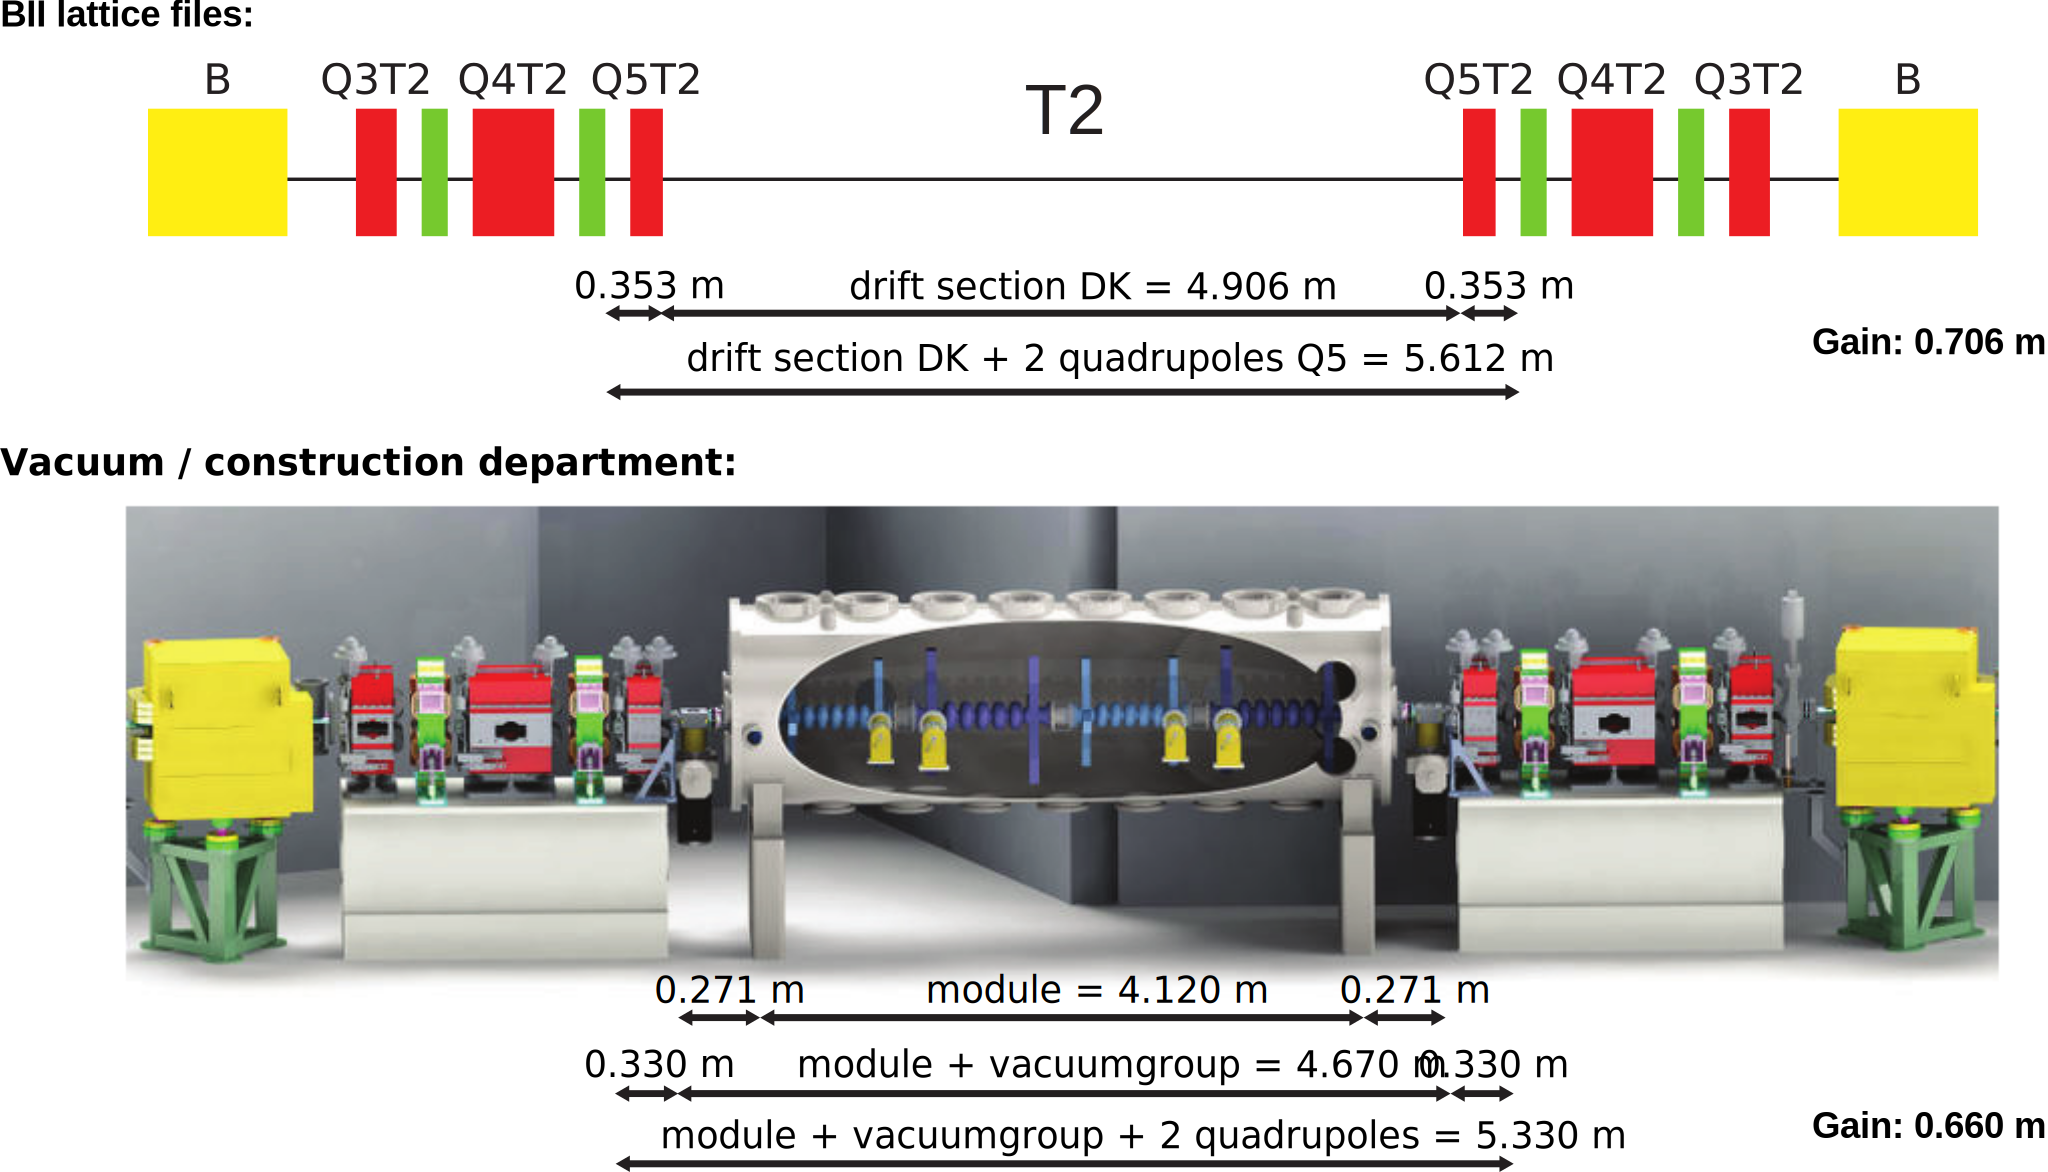
\includegraphics[width = \textwidth]{images/01-cavity-in-T2.pdf}
	\caption[The cryomodule and the magnets of the T2 section.]{The cryomodule and the magnets of the T2 section (dipole-yellow, quadruple-red, sextupole-green).}
	\label{fig:cavity-in-T2}
\end{figure}
\chapter{Transversal beam dynamics in circular accelerators} \label{chapter03}

% i build a python tool and explain at each step how i approached the physics

This chapter introduces the important methods and physics of transverse motion of particles in circular accelerators. This thesis only considers the linear order of beam optics, which are called so in analogy to geometrical light optics. Its physical concepts were developed by Courant and Snyder~\cite{courantsnyder}. The following introduction to linear beam optics forms the basis of my python tool.

The books from Klaus Wille~\cite{wille}, Frank Hinterberger~\cite{hinterberger} and Helmut Wiedemann~\cite{wiedemann} are the key sources for this chapter. However the notation and conventions will slightly differ to match the Elegant~\cite{elegant} style, which I used as main reference for my simulations.

\section{Equation of motion of charged particles in magnetic fields}
In this section the equations of motion for linear beam optics are derived. The fundamental force on a particle with the charge $q$ and velocity $v$ is called the \textit{Lorentz force}:
\begin{equation}
	\begin{aligned}[b]
		\textbf{F}_{\textup{L}} = \textbf{F}_\textup{E} + \textbf{F}_\textup{B} = q \: \textbf{E} + q \: \textbf{v} \times \textbf{B}.
	\end{aligned}\label{lorentzforce}
\end{equation}
As an electron in a modern synchrotron radiation source is moving almost with the speed of light~$c_0$ only the magnetic part $\textbf{F}_\textup{B}$ is of particular interest in the following. Electric fields with an effect in the same magnitude are technically not feasible.

The first subsection introduces the standard coordinate system of accelerator physics, which minimizes the mathematical efforts and which is especially helpful for the multipole expansion of the magnetic field in the second subsection. The linear approximation of the equations of motion in the third subsection is the essential foundation for the transfer matrix method in the next section.

\subsection{The co-moving coordinate system}
\begin{figure}
	\centering
	\includegraphics[width = 0.8\textwidth]{images/03-comoving-cartesian-coordinates.pdf}
	\caption{Co-moving curvilinear Frenet-Serret coordinates.}
	\label{fig:comovingcoordinates}
\end{figure}
The ideal beam trajectory in an accelerator is defined by the position and design of its beam guiding magnets. This perfect trajectory is called the \textit{orbit}. It is useful to describe the motion of a particle in relation to it. Therefore we introduce the orthogonal coordinate system $K = (x,y,s)$ whose origin follows along the orbit. This curvilinear coordinate system with the basis vectors
\begin{equation}\begin{aligned}[b]
		 & \uvec{s}(s)= \frac{\du \textbf{r}_0(s)}{\du s} &  & \small\text{unit vector tangent to the orbit} \\
		 & \uvec{x}(s)                                    &  & \small\text{normal (horizontal) unit vector}  \\
		 & \uvec{y}(s)= \uvec{s}(s) \times \uvec{x}(s)    &  & \small\text{binormal (vertical) unit vector}
	\end{aligned}\label{frenetserretvectors}\end{equation}
is also known as \textit{Frenet-Serret system}. While the \textit{s}-axis moves tangential to the orbit, the \textit{x-y} plane is perpendicular to it. The $s$ coordinate is defined by the distance covered on the orbit. The $z$ coordinate corresponds to the path length of the individual particle trajectory. The horizontal and vertical coordinates are labeled with $x$ and $y$. For statements which are valid for both transversal planes we will use the general variable $u$. The horizontal and vertical radii of curvature of the orbit are identified with $\rho_\text{0x}$ and $\rho_\text{0y}$\footnote{In our definition of the Frenet-Serret system the \textit{x}-axis points to the left of the beam direction. Therefore the horizontal and vertical radius of curvature for a particle bended to the right in the direction of travel is positive and vice versa. It is also common to define the \textit{x}-axis so that it points to the right. In such a coordinate system the sign of the curvature would change.}. Accordingly $\kap = \rho_\text{0x}^{-1}$ and $\kapy = \rho_\text{0y}^{-1}$ are the horizontal and vertical curvatures of the orbit, respectively.
\begin{figure}
	\centering
	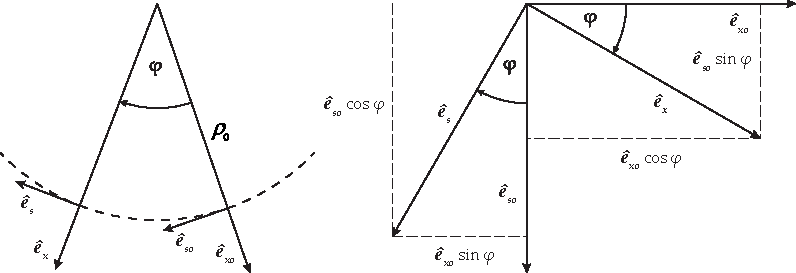
\includegraphics[width = 0.95\textwidth]{images/03-rotation-of-the-coordinate-system.pdf}
	\caption{Rotation of the Frenet-Serret frame around the y-axis.}
	\label{fig:rotationofcoordinates}
\end{figure}

The position of the individual particle in the laboratory frame\footnote{The Frenet-Serret frame is a non-intertial reference frame. To avoid the complexitiy of general relativity it is necessary to add the position of the coordinate origin $\textbf{r}_0(s)$.}  is given as the sum of its coordinates in the Frenet-Serret system and of the orbit position $\textbf{r}_0(s)$
\begin{equation}\textbf{r}(x,y,s) =  \textbf{r}_0(s) + x(s) \: \uvec{x}(s) + y(s) \: \uvec{y}(s).\label{positionvector}\end{equation}
To derive the equations of motion due to the Lorentz force we have to get the first and second time derivatives of the position vector $\textbf{r}$. As the orbit position~\textit{s} of a particle is clearly defined for each time~\textit{t}, we can choose \textit{s} as independent variable. The orbit position vector $\textbf{r}_0$ changes with $\du \textbf{r}_0 = \uvec{s} \: \du s$. Using the chain rule the first time derivative of (\ref{positionvector}) can be written as
\begin{equation}\begin{aligned}[b]
		\dot{\textbf{r}} = \frac{\du \textbf{r}}{\du s} \frac{\du s}{\du t} = \dfrac{\du x}{\du s} \: \dot{s} \: \uvec{x} + x \: \dot{s} \: \dfrac{\du \uvec{x}}{\du s} + \dfrac{\du y}{\du s} \: \dot{s} \: \uvec{y} + y \:\dot{s}\: \dfrac{\du \uvec{y}}{\du s}+ \dot{s} \: \uvec{s}.
	\end{aligned}\label{timediffpositionvector}\end{equation}
The change of the basis vectors is exemplary shown for the horizontal plane in \autoref{fig:rotationofcoordinates}. The geometric relation of rotation angle $\varphi_\textup{x0}$ to the tangential vector $\uvec{s}$ and to the normal vector~$\uvec{x}$ is given by:
\begin{equation}\begin{aligned}[b]
		\uvec{x} \quad & =\quad \cos{\varphi} \: \uvec{x0} + \sin{\varphi}\: \uvec{s0} \\
		\uvec{s} \quad & =\quad -\sin{\varphi} \: \uvec{x0}+ \cos{\varphi}\: \uvec{s0}
	\end{aligned}\label{unitvectors}\end{equation}
There is an analogous relation for the vertical plane. With the horizontal and vertical deflecting angles of the orbit
\begin{equation}\begin{aligned}[b]
		\du\varphi_{\textup{x}0} & = \kappa_{\textup{x}0} \: \du s   \\
		\du\varphi_{\textup{y}0} & = \kappa_{\textup{y}0} \: \du s .
	\end{aligned}\label{difforbitposition}\end{equation}
we can write down the derivative of the basis vectors with respect to the orbit position $s$:
\begin{equation}\begin{aligned}[b]
		\frac{\du \uvec{x}(s)}{\du s} & = \frac{\du \varphi_\textup{x0}}{\du s}  \frac{\du \uvec{x}}{\du \varphi_\textup{x0}} = \kap \: \uvec{s}(s)                                                                                                                          \\
		\frac{\du \uvec{y}(s)}{\du s} & = \frac{\du \varphi_\textup{y0}}{\du s}  \frac{\du \uvec{y}}{\du \varphi_\textup{y0}} = \kappa_{\textup{y}0} \: \uvec{s}(s)                                                                                                          \\
		\frac{\du \uvec{s}(s)}{\du s} & = \frac{\du \varphi_\textup{x0}}{\du s}  \frac{\du \uvec{s}}{\du \varphi_\textup{x0}} + \frac{\du \varphi_\textup{y0}}{\du s}  \frac{\du \uvec{s}}{\du \varphi_\textup{y0}}=- \kap \uvec{x}(s) - \kappa_{\textup{y}0} \: \uvec{y}(s)
	\end{aligned}\label{difffrenetserretvectors}\end{equation}
Substitution of (\ref{difffrenetserretvectors}) into (\ref{timediffpositionvector}) and using $h = 1 + \kap x + \kapy y$ yields
\begin{equation}\begin{aligned}[b]
		\dot{\textbf{r}} =x' \dot{s} \: \uvec{x} + y' \dot{s} \: \uvec{y} +  h \;\dot{s} \: \uvec{s}.
	\end{aligned} \label{frenetserretvelocity}\end{equation}
Here the derivative with respect to $s$ is denoted with the prime symbol. The second time derivative of the position vector can be derived by using the chain rule again $\ddot{\textbf{r}} = \frac{\du \dot{\textbf{r}}}{\du s} \frac{\du s}{\du t}$\footnote{We assume $\dot{\kappa}_\textup{x0} = \dot{\kappa}_\textup{y0} = 0$.}:
\begin{equation}\begin{aligned}[b]
		\ddot{\textbf{r}} = \left(x''\dot{s}^2 + x' \ddot{s} - h \kap \dot{s}^2\right) \uvec{x} +  \left(y'' \dot{s}^2 + y' \ddot{s} - h \kapy \dot{s}^2\right)  \uvec{y} + \left(2 \kap x'\dot{s}^2+ 2\kapy y'\dot{s}^2+h \ddot{s}\right) \uvec{s},
	\end{aligned}\label{frenetserretacceleration}\end{equation}
With the equations (\ref{frenetserretvelocity}) and (\ref{frenetserretacceleration}) we found the representation of the velocity and acceleration of a particle in our new coordinate system. Due to the introduction of the co-moving Frenet-Serret system we have coordinates which are directly related to the particles deviations from the orbit.

%As the size and divergence of the beam are very small, this formalism allows us to do linear beam optics.



\subsection{Multipole expansion of the magnet field}
When steering a charged particle in an accelerator the Lorentz force supplies the centripetal force
\begin{equation}\begin{aligned}[b]
		\textbf{F}_{\textup{centripetal}} \eq \textbf{F}_{\textup{Lorentz}} \\
		- m \: v^2 \: \boldsymbol{\kappa} \: \eq  q \: (\textbf{v} \times \textbf{B}).
	\end{aligned}\label{radiusofcurvature}\end{equation}
Here the mass $m$ corresponds to the relativistic mass. $\boldsymbol\kappa = (\kappa_\textup{x},\kappa_\textup{y},\kappa_\textup{s} \approx 0)$ is the curvature of the particle trajectory.
As we restrict us to purely transversal magnetic fields and as the transversal velocity components of a relativistic particle beam are small compared to its velocity
\begin{equation}
	v_{\textup{x}}\ll v, \: v_{\textup{y}}\ll v, \: v_{\textup{z}} \approx v,
\end{equation}
$p_\textup{z}$ equals with good approximation $p$. Thus from (\ref{radiusofcurvature}) the horizontal and vertical curvatures are given by\footnote{The sign comes due to the convention of the Frenet-Serret coordinates.}
\begin{equation}\begin{aligned}[b]
		\kappa_\textup{x} \: (x,y,s,p) \eq \dfrac{q}{p} B_{\textup{y}}(x,y,s)     \\
		\kappa_\textup{y} \: (x,y,s,p) \eq - \dfrac{q}{p} B_{\textup{x}}(x,y,s) . \\
	\end{aligned}\label{horizontalradiusofcurvature}\end{equation}
As the magnetic field could be an arbitrary function it is useful to simplify it further. An appropriate approach is to expand the magnetic field into a sum of multipoles. In theory this is possible for any magnetic field. Due to the Frenet-Serret frame we are able to expand the magnetic field at the orbit $x_0 = y_0 = 0$. For the vertical magnetic field along the x-axis this leads to
\begin{figure}
	\centering
	\includegraphics[width = \textwidth]{images/03-multipole-types-4.pdf}
	\caption[The different multipoles and their field lines.]{The different multipoles and their field lines. In the upper row the magnetic fields are produced due to the arrangement of electric currents. The field lines below are the pure components of the multipole expansion. The bottom row shows the vertical magnetic field B$_\textup{y}$ along the x-axis at $y = 0$. Here the graph of real multipole corresponds to the black solid line. The graph of  the respective expansion term is marked with a red dashed line.}
	\label{fig:multipoletypes}
\end{figure}

\begin{equation}\begin{aligned}[b]
		B_y(x,y=0) \quad & =\quad  B_{y0} \quad                      & + & \quad \dfrac{\du B_y}{\du x}x \quad  & + & \quad \dfrac{1}{2}\dfrac{\du^2 B_y}{\du x^2}x^2 \quad & + & \quad \dfrac{1}{6}\dfrac{\du^3 B_y}{\du x^3}x^3 \quad & + & \quad  ... \; . \\
		                 & \quad \quad \: \footnotesize\text{dipole} &   & \quad \footnotesize\text{quadrupole} &   & \quad\: \footnotesize\text{sextupole}                 &   & \quad\: \footnotesize\text{octupole}                  &   &
	\end{aligned}\label{multipoleexpansion}\end{equation}
Each term can be identified with a multipole. The ideal dipole field has only a non zero dipole component. For the perfect quadrupole only the linear term is non zero, etc. The simplest way to realize the first four multipoles is shown in \autoref{fig:multipoletypes}. It can be observed that the electric wires cause an magnetic field which in the inside corresponds to the particular term of the expansion. With the transition to the outer areas the discrepancies  compared to the ideal multipoles increases. In practice there a certain techniques to extend the useful field regions. For accelerators it is common to use another configuration of the coils. Furthermore the magnetic field is enhanced by iron yokes.

By substituting (\ref{multipoleexpansion}) into (\ref{radiusofcurvature}) it follows that
\begin{equation}\begin{aligned}[b]
		\kappa_\textup{x}(x,p) \quad & =\quad  \frac{q}{p}B_{y0} \quad      & + & \quad  \frac{q}{p}\dfrac{\du B_y}{\du x}x \quad & + & \quad  \dfrac{1}{2}\frac{q}{p}\dfrac{\du^2 B_y}{\du x^2}x^2 \quad & + & \quad \dfrac{1}{6}\frac{q}{p}\dfrac{\du^3 B_y}{\du x^3}x^3 \quad & + & \quad  ...    \\
		\quad                        & =\quad \kappa_{\textup{x0}}(p) \quad & + & \quad k(p)  x \quad                             & + & \quad \frac{1}{2} m(p) x^2 \quad                                  & + & \quad \frac{1}{6} o(p) x^3 \quad                                 & + & \quad ... \;. \\
	\end{aligned}\label{magneticfieldexpansion}\end{equation}
There is an equivalent expression for the vertical plane. We can observe that the curvature of the trajectory only depends on the strength of the respective multipole and the transversal coordinates. Consequently the movement of a particle with a small offset to the orbit is dominated by the lower order terms. Only taking dipoles and quadrupoles into account is called \textit{linear beam optics}. The most important multipoles and general effects on the particle trajectory are listed in Table \ref{tabledifferentmultipoles}.
\begin{table}
	\caption{The different types of magnets and their general effect on the particle motion.}
	\centering
	\begin{tabular}{l l l}
		\toprule
		\textbf{magnet type} & \textbf{term}                                           & \textbf{effect}                     \\
		\midrule
		dipole               & $\kap = \frac{q}{p} B_{\textup{y}}$                     & particle bending along a given path \\
		quadrupole           & $ k = \frac{q}{p} \frac{\du B_{\textup{y}}}{\du x}$     & transversal focusing                \\
		sextupole            & $ m = \frac{q}{p} \frac{\du^2 B_{\textup{y}}}{\du x^2}$ & compensation of chromaticity        \\
		\bottomrule                                                                                                          \\
	\end{tabular}
	\label{tabledifferentmultipoles}
\end{table}



\subsection{Formulating the equations of motion in linear beam optics}
Now we can formulate the equations of motion. The magnetic part of the Lorentz force (\ref{lorentzforce}) can be written as
\begin{equation}\begin{aligned}[b]
		\ddot{\textbf{r}} \eq \frac{q}{m} \: (\dot{\textbf{r}} \times \textbf{B}) .
	\end{aligned}\label{magneticlorentz}\end{equation}
With substituting the first (\ref{frenetserretvelocity}) and second (\ref{frenetserretacceleration}) time derivative of the position vector in \eqref{magneticlorentz} we obtain
\begin{equation}\begin{aligned}[b]
		x''\dot{s}^2 + x' \ddot{s} - h \; \kappa_{\textup{x}0} \;\dot{s}^2 \quad  & =\quad -\frac{q}{m} B_\textup{y}  h \dot{s} \\
		y'' \dot{s}^2 + y' \ddot{s} - h \; \kappa_{\textup{y}0} \;\dot{s}^2 \quad & =\quad \frac{q}{m} B_\textup{x}  h \dot{s}.
	\end{aligned}\label{eom1}\end{equation}
These are the equations of motion for a charged particle. There are no approximations made so far. In principle we could numerical integrate \eqref{eom1} and would obtain the particle trajectory. The advantage of linearizing the equations of motion is that we can develop a formalism with analytic quantities which describe the beam dynamics.

As shown in \autoref{fig:pathlengthdiff} the relation between the orbit length and the particle trajectory is in linear approximation given by
\begin{figure}
	\centering
	\includegraphics[width = .7\textwidth]{images/03-path-length-difference_new.pdf}
	\caption{Difference in path length between orbit and particle trajectory.}
	\label{fig:pathlengthdiff}
\end{figure}
%\begin{SCfigure}[50]
%	\includegraphics[width = .38\textwidth]{images/03-path-length-difference_new.pdf}
%	\caption{Difference in path length between orbit and particle trajectory.}
%	\label{fig:pathlengthdiff}
%\end{SCfigure}
\begin{equation}\begin{aligned}[b]
		\du z = (1 + \kappa_{\textup{x}0} x) \du s + \mathcal{O}\left(2\right).
	\end{aligned}\label{pathdiff}\end{equation}
With  $v = \frac{\du z}{\du t}$  the momentum of a particle  $p$ can be written as
\begin{equation}\begin{aligned}[b]
		p = mv \approx m (1 + \kappa_{\textup{x}0} x) \; \dot{s} = m h \dot{s}.
	\end{aligned}\label{vecapprox}\end{equation}
Apart from velocity changes, the second time derivate of the orbit coordinate of a particle is effected by two aspects. First an offset in a bending section leads to a different path length and $\dot{s}$ changes. This complies to the first term in (\ref{pathdiff}). Secondly a particle with an angle divergence to the orbit travels in a slightly different direction. Here $\dot{s}$ decreases. This corresponds to the higher order terms in (\ref{pathdiff}). As the transversal velocity components of a relativistic particle beam are small compared to its longitudinal components, the offset changes slowly. Therefore the second time derivative of the orbit position is negligible and we can assume
\begin{equation}\begin{aligned}[b]
		\ddot{s} \approx 0.
	\end{aligned}\label{secondtimederivativeorbit}\end{equation}
Due to the Lorentz factor $\gamma$ equally fast particles in a relativistic bunch can have small discrepancies in momentum. Therefore it is useful to define the relative momentum error $\delta = \frac{\Delta p}{p_0}$ from the nominal momentum $p_0$. As these deviations are still small we can expand the momentum $p$ at $p_0$ in $\delta$ up to the linear order
\begin{equation}\begin{aligned}[b]
		\frac{1}{p} = \frac{1}{p_0}\frac{1}{1+\delta} = \frac{1}{p_0} (1 -\delta + \mathcal{O}(2)) .
	\end{aligned}\label{momentumexpansion}\end{equation}
Applying (\ref{vecapprox}), (\ref{secondtimederivativeorbit}) and (\ref{momentumexpansion}) to (\ref{eom1}) yields
\begin{equation}\begin{aligned}[b]
		x'' - \left( 1 +\kappa_{\textup{x}0} x \right)\kappa_{\textup{x}0}  \quad & =\quad - \left(1 - \delta\right) \left(\kappa_{\textup{x}0} + k x \right) \left( 1 +\kappa_{\textup{x}0} x \right)^2 \\
		y'' \quad                                                                 & =\quad \left(1 - \delta\right) k  \left( 1 +\kappa_{\textup{x}0} x\right)^2 .
	\end{aligned}\label{eom_2}\end{equation}
By multiplying all parentheses while retaining only linear and quadratic terms in $x$, $y$ and $\delta$ we obtain
\begin{equation}\begin{aligned}[b]
		x''(s) + \left[ \kappa_{\textup{x}0}^2(s) + k(s) \right] x(s) \quad & =\quad \kappa_{\textup{x}0} \: \delta \\
		y''(s) - k(s) \; y(s) \quad                                         & =\quad 0 .
	\end{aligned}\label{lineareom}\end{equation}
These are the equations of motion in linear order. They are the foundation for my python tool.



\section{The transfer matrices of the hard-edge model} \label{sectiontransfermatrix}
To describe the full motion of a single particle in the three dimensional space six phase space coordinates are needed. Instead of the most common set of coordinates $(x,y,z,p_\textup{x},p_\textup{x},p_\textup{z})$ we are using
\begin{equation}\begin{aligned}[b]
		\textbf{X}(s) =
		\begin{pmatrix}
			x(s) \\ x'(s) \\ y(s) \\ y'(s) \\ l(s) \\ \delta(s)
		\end{pmatrix}
		=
		\begin{pmatrix}
			\textup{horizontal offset} \\ \textup{horizontal slope} \\ \textup{vertical offset}\\ \textup{vertical slope} \\ \textup{longitudinal offset}  \\ \textup{relative momentum error}
		\end{pmatrix},
	\end{aligned}\label{particlevector}\end{equation}
where, as we did not a Lorentz transformation, all coordinates are measured in the laboratory frame. Due to the linear approximation of the equations of motion the transition from initial coordinate vector $\textbf{X}(s)$  to that one after any arbitrary path length $\textbf{X}(s+L)$ can be represented by the matrix multiplication
\begin{equation}\begin{aligned}[b]
		\textbf{X}(s+L) = \textbf{R}(s,s+L) \cdot\textbf{X}(s).
	\end{aligned}\label{rmatrixmultiplication}\end{equation}
Here $\textbf{R}(s)$ corresponds to the $6 \times6$-dimensional transfer matrix.  Our task is now to find the matrix representations for the particular element sections, especially for the drift space, dipole and quadrupole.

The entries for transversal offset $u(s)$ and slope $u'(s)$ can be found by solving (\ref{lineareom}). The longitudinal offset $l(s)$ is mainly changed by two effects. Firstly it depends on the difference between the trajectory length $Z$ and orbit length $L$ in the particular element. With the linear approximation from (\ref{pathdiff}) we find for the path length $Z = \int_0^s (1 +\kap x )\du s$. Secondly the time for a particle with different velocity on the same path is scaled by the factor $\frac{\Delta v}{v_0}$. For the longitudinal offsets we obtain
\begin{equation}\begin{aligned}[b]
		l(s) \quad & =\quad l_0 -(Z-L) + L\frac{\Delta v}{v_0}                               \\
		           & \approx\quad l_0 - \int_0^s \kap x \du s + \frac{L}{\gamma^2} \delta_0,
	\end{aligned}\label{logitudinaloffsettchange}\end{equation}
where we used the approximation $\frac{\Delta v}{v_0}\approx\frac{1}{\gamma^2}\frac{\Delta p}{p_0}$ from relativistic kinematics:
\begin{equation}\begin{aligned}[b]
		\frac{\du p}{\du v} = m_0 \gamma + m_0 \frac{v^2}{c^2} \gamma^3 = m_0 \gamma^3 (\frac{1}{\gamma^2} + \frac{v^2}{c^2}) = m_0 \gamma^3 = \frac{p}{v} \gamma^2
	\end{aligned}\label{relativistickinematicseq}\end{equation}
Without radiation and external influences the momentum of a particle stays constant. Hence the trivial equation for the relative momentum offset
\begin{equation}\begin{aligned}[b]
		\delta(s)  = \delta(0) = \delta_0
	\end{aligned}\label{momentumchange}\end{equation}
leads to a bottom row of the transfer matrix, where only one entry is nonzero.
\subsection*{Drift space}
For the drift space $\kap(s) = k(s) = 0$, therefore (\ref{lineareom}) simplifies to
\begin{equation}\begin{aligned}[b]
		x''(s) \quad & =\quad 0      \\
		y''(s)\quad  & =\quad 0 \: ,
	\end{aligned}\label{drifteom}\end{equation}
which is a  homogeneous second order linear differential equations. With the initial conditions for both transversal planes $(u(0) = u_0, u'(0) = u_0')$, this is satisfied by
\begin{equation}\begin{aligned}[b]
		u(s) \quad & =\quad 1 \cdot u_0 +s\cdot u'_0        \\
		u'(s)\quad & =\quad  0 \cdot u_0 +1 \cdot u'_0 \: .
	\end{aligned}\label{drifteomsolved}\end{equation}
As the orbit in the drift space and quadrupole has no curvature, from (\ref{logitudinaloffsettchange}) it follows that
\begin{equation}\begin{aligned}[b]
		l(s) \quad & =\quad l_0 + \frac{L}{\gamma^2} \delta_0 \: .
	\end{aligned}\label{driftlength}\end{equation}
With (\ref{drifteomsolved}),(\ref{driftlength}) and (\ref{momentumchange}) the transfer matrix of the drift space is given by
\begin{equation}\begin{aligned}[b]
		\textbf{R}_{\textup{drift}} =
		\begin{pmatrix}
			1 & L & 0 & 0 & 0 & 0          \\
			0 & 1 & 0 & 0 & 0 & 0          \\
			0 & 0 & 1 & L & 0 & 0          \\
			0 & 0 & 0 & 1 & 0 & 0          \\
			0 & 0 & 0 & 0 & 1 & L/\gamma^2 \\
			0 & 0 & 0 & 0 & 0 & 1
		\end{pmatrix}.
	\end{aligned}\label{driftmatrix}\end{equation}

\subsection*{Dipole magnet}
For the solution of (\ref{lineareom}) for the dipole and quadrupole we assume a constant field along the longitudinal magnet axis. This approximation of a Heaviside function shaped field is known as the \textit{hard edge model}. With $\kap(s) = const$ and $k(s) = 0$ in the dipole magnet we obtain

\begin{equation}\begin{aligned}[b]
		x''(s) + \kappa_{\textup{x}0}^2 x(s) \quad & =\quad \kappa_{\textup{x}0} \: \delta \\
		y''(s) \quad                               & =\quad 0 \: .
	\end{aligned}\label{dipoleom}\end{equation}
The solution of the vertical plane $y(s)$ corresponds to that one of the drift space. For the horizontal plane we have a inhomogeneous second order linear differential equation. Here the solution is given by the sum of the complementary and the particular solution $x(s) = x_\textup{homo} + x_\textup{part}$. The homogeneous part corresponds to the harmonic oscillator
\begin{equation}\begin{aligned}[b]
		x_\textup{homo} = C_1 \cos{\kap s} + C_2 \sin{\kap s}.
	\end{aligned}\label{harmonicosci}\end{equation}
As the inhomogeneous part of (\ref{dipoleom}) is constant, for the particular solution it follows that
\begin{equation}\begin{aligned}[b]
		x_\textup{part} = const \quad\rightarrow\quad x_\textup{part} \kap^2 = \delta \kap \quad\rightarrow\quad x_\textup{part} = \frac{\delta}{\kap} \: .
	\end{aligned}\label{dipoleompart}\end{equation}
With the initial conditions $(x(0) = x_0, x'(0) = x_0')$ and deflection angle $\varphi_0 = \kap s$ the solution of the horizontal plane is given by
\begin{equation}\begin{aligned}[b]
		x(s) \quad  & =\quad \cos{\varphi_0}       &  & \cdot x_0 & +\quad & \frac{1}{\kap}\sin{\varphi_0} &  & \cdot x_0' & +\quad & \frac{1}{\kap}(1-\cos{\varphi_0}) &  & \cdot \delta_0      \\
		x'(s) \quad & =\quad -\kap \sin{\varphi_0} &  & \cdot x_0 & +\quad & \cos{\varphi_0}               &  & \cdot x_0' & +\quad & \sin{\varphi_0}                   &  & \cdot \delta_0 \: .
	\end{aligned}\label{dipoleomsolved}\end{equation}
By substituting (\ref{dipoleomsolved}) into (\ref{logitudinaloffsettchange}) the longitudinal offset can be calculated by
\begin{equation}\begin{aligned}[b]
		l(s) = l_0 -\sin{\varphi_0} \cdot x_0 -\frac{1}{\kap}(1-\cos{\varphi_0}) \cdot x_0 ' + \left( \frac{\varphi_0}{\kap \gamma^2} - \frac{1}{\kap}(\varphi_0 - \sin{\varphi_0})\right) \cdot \delta_0 \: .
	\end{aligned}\label{dipoleomlength}\end{equation}
For the transfer matrix of the dipole magnet we obtain
\begin{equation}\begin{aligned}[b]
		\textbf{R}_{\textup{sector dipole}} =
		\begin{pmatrix}
			\cos{\varphi_0}        & \frac{1}{\kap}\sin{\varphi_0}      & 0 & 0 & 0 & \frac{1}{\kap}(1-\cos{\varphi_0})                                             \\
			- \kap \sin{\varphi_0} & \cos{\varphi_0}                    & 0 & 0 & 0 & \sin{\varphi_0}                                                               \\
			0                      & 0                                  & 1 & L & 0 & 0                                                                             \\
			0                      & 0                                  & 0 & 1 & 0 & 0                                                                             \\
			-\sin{\varphi_0}       & -\frac{1}{\kap}(1-\cos{\varphi_0}) & 0 & 0 & 1 & \frac{\varphi_0}{\kap \gamma^2} - \frac{1}{\kap}(\varphi_0 - \sin{\varphi_0}) \\
			0                      & 0                                  & 0 & 0 & 0 & 1
		\end{pmatrix}
	\end{aligned}\label{dipolmatrix}\end{equation}
This is the transfer matrix for a sector dipole, which is shaped the way that its entrance and exit areas are perpendicular to the orbit. For several design reasons often rectangular dipoles are used. As they change the entrance and exit edge angle, this influences the trajectory for particles with a transversal offset. Due to geometrical considerations (see \autoref{appendixedgefocusing}) this effect known as \textit{edge focusing} can be expressed by the matrix
\begin{equation}\begin{aligned}[b]
		\textbf{R}_{\textup{edge}} =
		\begin{pmatrix}
			1                 & 0 & 0                  & 0 & 0 & 0 \\
			\kap \tan{\alpha} & 1 & 0                  & 0 & 0 & 0 \\
			0                 & 0 & 1                  & 0 & 0 & 0 \\
			0                 & 0 & -\kap \tan{\alpha} & 1 & 0 & 0 \\
			0                 & 0 & 0                  & 0 & 1 & 0 \\
			0                 & 0 & 0                  & 0 & 0 & 1
		\end{pmatrix} \: ,
	\end{aligned}\label{edgematrix}\end{equation}
where $\alpha$ corresponds to angle difference from a sector dipole. The transfer matrix of a rectangular dipole is given by
\begin{equation}
	\textbf{R}_{\textup{rectangular dipole}} = \textbf{R}_{\textup{edge}} \cdot \textbf{R}_{\textup{sector dipole}} \cdot \textbf{R}_{\textup{edge}} \: .
\end{equation}
\begin{figure}
	\centering
	\includegraphics[width = .5\textwidth]{images/03-weak-focusing.pdf}
	\caption{Weak focusing of a dipole magnet.}
	\label{fig:weakfocusing}
\end{figure}


\subsection*{Quadrupole magnet}
With $\kap(s) = 0$ and $k(s) = const$ for the quadrupole magnet (\ref{lineareom}) yields
\begin{equation}\begin{aligned}[b]
		x''(s) + k x(s) \quad & =\quad 0      \\
		y''(s) - k x(s)\quad  & =\quad 0 \: .
	\end{aligned}\label{quadeom}\end{equation}
This is a homogeneous second order differential equation and has the same solution like the complementary part of the dipole. For the horizontal focusing quadrupole $k > 0$ this is satisfied by
\begin{equation}\begin{aligned}[b]
		x(s) \quad  & =\quad  \cos{\sqrt{k}s}          &  & \cdot x_0 & +\quad & \frac{1}{\sqrt{k}}\sin{\sqrt{k}s}  &  & \cdot x_0'   \\
		x'(s) \quad & =\quad -\sqrt{k}\sin{\sqrt{k}s}  &  & \cdot x_0 & +\quad & \cos{\sqrt{k}s}                    &  & \cdot x_0'\: \\
		y(s) \quad  & =\quad \cosh{\sqrt{k}s}          &  & \cdot y_0 & +\quad & \frac{1}{\sqrt{k}}\sinh{\sqrt{k}s} &  & \cdot y_0'   \\
		y'(s) \quad & =\quad  \sqrt{k}\sinh{\sqrt{k}s} &  & \cdot y_0 & +\quad & \cosh{\sqrt{k}s}                   &  & \cdot y_0' .
	\end{aligned}\label{quadeomsolved}\end{equation}
The longitudinal solution of the quadrupole magnet is analogous to the drift space. The transfer matrix for the horizontal focusing quadrupole can be written:
\begin{equation}\begin{aligned}[b]
		\textbf{R}_{\textup{quadrupole,v}} =
		\begin{pmatrix}
			\cos{\sqrt{k}L}          & \frac{1}{\sqrt{k}}\sin{\sqrt{k}L} & 0                        & 0                                  & 0 & 0          \\
			-\sqrt{k}\sin{\sqrt{k}L} & \cos{\sqrt{k}L}                   & 0                        & 0                                  & 0 & 0          \\
			0                        & 0                                 & \cosh{\sqrt{k}L}         & \frac{1}{\sqrt{k}}\sinh{\sqrt{k}L} & 0 & 0          \\
			0                        & 0                                 & \sqrt{k}\sinh{\sqrt{k}L} & \cosh{\sqrt{k}L}                   & 0 & 0          \\
			0                        & 0                                 & 0                        & 0                                  & 1 & L/\gamma^2 \\
			0                        & 0                                 & 0                        & 0                                  & 0 & 1          \\
		\end{pmatrix}
	\end{aligned}\label{quadrupolematrixhorizontal}\end{equation}
The transfer matrix for the vertical focusing quadrupole results from swapping the transversal block matrices and using the absolute value of $|k|$:
\begin{equation}\begin{aligned}[b]
		\textbf{R}_{\textup{quadrupole,h}} =
		\begin{pmatrix}
			\cosh{\sqrt{k}L}         & \frac{1}{\sqrt{k}}\sinh{\sqrt{k}L} & 0                        & 0                                 & 0 & 0          \\
			\sqrt{k}\sinh{\sqrt{k}L} & \cosh{\sqrt{k}L}                   & 0                        & 0                                 & 0 & 0          \\
			0                        & 0                                  & \cos{\sqrt{k}L}          & \frac{1}{\sqrt{k}}\sin{\sqrt{k}L} & 0 & 0          \\
			0                        & 0                                  & -\sqrt{k}\sin{\sqrt{k}L} & \cos{\sqrt{k}L}                   & 0 & 0          \\
			0                        & 0                                  & 0                        & 0                                 & 1 & L/\gamma^2 \\
			0                        & 0                                  & 0                        & 0                                 & 0 & 1
		\end{pmatrix}
	\end{aligned}\label{quadrupolematrixvertical}\end{equation}
We are now able to calculate the trajectory of a particle through any arbitrary number $N$ of magnets:
\begin{equation}
	\textbf{X}(s+L) = \textbf{R}_N\cdot ... \cdot\textbf{R}_2 \cdot \textbf{R}_1 \cdot \textbf{X}(s)
\end{equation}

\section{Twiss parameters (Courant-Snyder functions)}
The in \autoref{sectiontransfermatrix} derived transfer matrices method is in principle possible for any desired number of particles, but is very impractical for many particles and allows only numerical investigations. Therefore it would be useful to have an analytical formalism for the entire beam. Such a description were develop by Courant and Synder~\cite{courantsnyder} and is given by the \textit{Courant-Synder functions}. These, also called \textit{Twiss parameters}, can be obtained by separating the effects of on- and off-momentum motion.

Therefore we first solve the linear equations of motion (\ref{lineareom}) for the \textit{dispersion-free} case. This leads us to the fundamental value of transversal beam motion, the \textit{beta function} $\beta(s)$. Afterwards we introduce the \textit{dispersion function} $\eta(s)$  to describe the influence of momentum deviations on the transversal motion. Off-momentum effects on the longitudinal path length are describe by the \textit{momentum compaction factor} $\alpha$.

\subsection{Betatron oscillation}
By neglecting the off-momentum terms and substituting $K(s) = \kappa_{\textup{x}0}^2(s) + k(s)$ for the horizontal and $K(s) = - k(s)$ for the vertical plane, the linear equations of motion \eqref{lineareom} simplify to
\begin{equation}\begin{aligned}[b]
		u''(s) + K(s) u(s) = 0,
	\end{aligned}\label{hillsequation}\end{equation}
where $u$ can be either $x$ or $y$. This, also known as \textit{Hill equation}, is a second-order linear ordinary differential equation, where the periodicity length of coefficient $K(s) = K(s + C)$ is given by the circumference $C$ of the orbit. According to \textit{Floquet's theorem} a solution of \eqref{hillsequation} can be written as product of a periodic function and an exponential function~\cite{Kuchment2012}. Hence the real part of the \textit{Floquet solution} is given by
\begin{equation}\begin{aligned}[b]
		u(s) = \sqrt{\epsilon} \sqrt{\beta(s)} \cos(\psi(s) + \psi_0),
	\end{aligned}\label{betatronoscillation}\end{equation}
where \textit{emittance} $\epsilon$ and initial phase $\psi_0$ are integration constants. Inserting (\ref{betatronoscillation}) and its second derivative into (\ref{hillsequation}) yields
\begin{equation}\begin{aligned}[b]
		\sqrt{\epsilon}\left( \frac{1}{2} \beta \beta'' - \frac{1}{4}\beta'^2 -\beta^2\psi'^2 + \beta ^2 K(s) \right)  \cos(\psi(s) + \psi_0) + \sqrt{\epsilon} \left( \beta' \psi' + \beta \psi'' \right)  \sin(\psi(s) + \psi_0) = 0 .
	\end{aligned}\label{betatronphase2}\end{equation}
As (\ref{betatronphase2}) must be true for all phases $\psi(s)$, we obtain the two relations
\begin{equation}\begin{aligned}[b]
		\frac{1}{2} \beta \beta'' - \frac{1}{4}\beta'^2 -\beta^2\psi'^2 + \beta ^2 K(s) = 0 \\
		\beta' \psi' + \beta \psi'' = 0 .
	\end{aligned}\label{betatronphase3}\end{equation}
Integrating the second equation twice and choosing the integration constant equal to one, leads us to the \textit{betatron phase}
\begin{equation}\begin{aligned}[b]
		\psi(s) = \int_0^s \frac{d \bar{s}}{\beta(\bar{s})}.
	\end{aligned}\label{betatronphase}\end{equation}
In circular accelerators the number of betatron oscillations per revolution
\begin{equation}\begin{aligned}[b]
		Q = \frac{1}{2 \pi}\int_s^{s+C} \frac{d \bar{s}}{\beta(\bar{s})}
	\end{aligned}\label{tune}\end{equation}
is called the \textit{tune}. As the initial betatron phase $\psi_0$ is different for each particle, there is always a particle which satisfies $\cos(\psi(s) + \psi_0) = \pm 1$. Consequently the \textit{envelope} of the particle beam is given by
\begin{figure}
	\centering
	\includegraphics[width = \textwidth]{images/03-envelope.pdf}
	\caption[Envelope of a particle beam.]{The envelope of a particle beam at the example of a FODO cell. The betatron oscillation for 33 electrons with an emittance of 5 nm rad is shown in the right graphic.}
	\label{fig:envelope}
\end{figure}
\begin{equation}\begin{aligned}[b]
		E(s) = \pm \sqrt{\epsilon} \sqrt{\beta(s)},
	\end{aligned}\label{Envelope}\end{equation}
where $\epsilon$ is the largest emittance of all particles. The function $\beta(s)$ is called the \textit{beta function} and is one of the \textit{Twiss parameter}. It is directly related to the transverse size of the entire beam and is therefore one of the most important quantities in circular accelerator physics. The meaning of the beta function for the single particle trajectory as well as for the trajectories of many particles is shown in \autoref{fig:envelope}.


\subsection{The phase space ellipse}
Differentiating (\ref{betatronoscillation}) with respect to the orbit position $s$ yields
\begin{equation}\begin{aligned}[b]
		u'(s) =  -\frac{\sqrt{\epsilon}}{\sqrt{\beta(s)}}  \left( \alpha(s) \cos(\psi(s) + \psi_0) + \sin(\psi(s) + \psi_0) \right),
	\end{aligned}\label{betatronoscillation2}\end{equation}
where we introduced the Twiss parameter $\alpha(s) := \frac{-\beta'(s)}{2}$ and used the relation $\psi'(s) = \frac{1}{\beta(s)}$. Rewriting (\ref{betatronoscillation}) and (\ref{betatronoscillation2}) as
\begin{equation}\begin{aligned}[b]
		\cos(\psi(s) + \psi_0) \quad & =\quad \frac{u(s)}{\sqrt{\epsilon}\sqrt{\beta(s)}}                                                          \\
		\sin(\psi(s) + \psi_0) \quad & =\quad \frac{\sqrt{\beta(s)}u'(s)}{\sqrt{\epsilon}} + \frac{\alpha(s) u(s)}{\sqrt{\epsilon}\sqrt{\beta(s)}}
	\end{aligned}\label{betatronoscillation3}\end{equation}
and using the Pythagorean trigonometric identity $\sin^2{\theta} + \cos^2{\theta} = 1$ leads us to
\begin{equation}\begin{aligned}[b]
		\frac{1 + \alpha^2(s)}{\beta(s)} u^2(s)  + 2 \alpha(s) u(s)u'(s) + \beta(s) u'^2(s) = \epsilon .
	\end{aligned}\label{betatronoscillation4}\end{equation}
With the introduction of another Twiss parameter $\gamma(s) := \frac{1 + \alpha^2(s)}{\beta(s)}$ (\ref{betatronoscillation4}) can be written as
\begin{equation}\begin{aligned}[b]
		\gamma(s) u^2(s) + 2 \alpha(s) u(s)u'(s) + \beta(s) u'^2(s) = \epsilon .
	\end{aligned}\label{phasespaceellipse}\end{equation}
This is the representation of an ellipse in the $u$-$u'$ phase space. Consequently the betatron oscillation of a particle with the transverse coordinates $(u,u')$ can be described by the movement along the continuous changing surface of an ellipse in phase space. The emittance $\epsilon$ is a constant of motion and is therefore also called \textit{Courant-Synder invariant}. This is in accordance with \textit{Liouville’s equation} (See \autoref{appendixliouvillestheorem})
\begin{equation}
	\frac{\du \rho(q,p,t)}{\du t} = 0
\end{equation}
and with the resulting \textit{Liouville's theorem}\footnote{Liouville's theorem was initially developed in statistical physics to describe the time evolution of a classical ensemble of systems in phase space. It is applicable to an electron beam due to the fact that a system of $N$ \textit{non-interacting} particles can be understood as a statistical ensemble. Furthermore the theorem is only valid for particles with the same Hamiltonian. This requirement is fulfilled in regard that all electrons are identical and see the same external magnetic fields.}, which states that the phase space distribution $\rho(q,p,t)$ of $N$ \textit{non-interacting} particles in conservatives systems is constant along any path. Thus their occupied volume $A = \pi \epsilon$ in phase space is conserved\footnote{Identical particles with the same Hamiltonian can not cross in phase space. Consequently the inner and outer points of any region $G$ cannot to propagate through the surface area $\partial G$. Thus the number of phase space points within $G$ stays constant. As the phase space distribution is constant, the phase space volume of $G$ must be conserved.}. As shown in \autoref{fig:phasespaceellipse} the shape of the phase space ellipse is defined by the Twiss parameters, what means that the motion of the entire beam can be described by the transformation of the Courant-Synder functions.

\begin{figure}
	\centering
	\includegraphics[width = \textwidth]{images/03-phase-space-ellipse-graphic.pdf}
	\caption[The phase space ellipse.]{The phase space ellipse is illustrated for two orbit positions $s_1$ and $s_2$. Due to the betatron oscillation a particle moves along the surface of the transforming ellipse. The position of an individual particle (red marked dot) is defined by the betatron phase $\psi(s)+ \psi_0$. The shape and size of the ellipse is determined by the Twiss parameters and by the Courant-Synder invariant.}
	\label{fig:phasespaceellipse}
\end{figure}


\subsection{Transformation of the Twiss parameters} \label{transformationofthetwissparameter}
To obtain the transformation of the phase space ellipse we write \eqref{phasespaceellipse} as
\begin{equation}\begin{aligned}[b]
		\begin{pmatrix}
			u(s) & u'(s)
		\end{pmatrix}
		\begin{pmatrix}
			\gamma(s) & \alpha(s) \\
			\alpha(s) & \beta(s)
		\end{pmatrix}
		\begin{pmatrix}
			u(s) \\
			u'(s)
		\end{pmatrix}
		= \epsilon .
	\end{aligned}\label{phasespaceellipse2}\end{equation}
With the \textit{beta matrix}
\begin{equation}\begin{aligned}[b]
		\textbf{B}(s) =
		\begin{pmatrix}
			\beta(s)   & -\alpha(s) \\
			-\alpha(s) & \gamma(s)
		\end{pmatrix}
	\end{aligned}\label{twissmartix}\end{equation}
and $\textbf{R} = \textbf{R}(s,L)$ we can write
\begin{equation}\begin{aligned}[b]
		\epsilon & = \textbf{X}^T(s) \textbf{B}^{-1}(s) \textbf{X}(s)                                                             \\
		         & = \textbf{X}^T(s) \textbf{R}^T (\textbf{R}^T)^{-1} \textbf{B}^{-1}(s) \textbf{R}^{-1} \textbf{R} \textbf{X}(s) \\
		         & = (\textbf{R} \textbf{X}(s) )^T (\textbf{R} \textbf{B}(s) \textbf{R}^T)^{-1} (\textbf{R} \textbf{X}(s))        \\
		         & = \textbf{X}^T(s+L) (\textbf{R} \textbf{B}(s) \textbf{R}^T)^{-1} \textbf{X}(s+L)                               \\
		         & \overset{!}{=} \textbf{X}^T(s+L) \textbf{B}^{-1}(s+L) \textbf{X}(s+L) ,
	\end{aligned}\label{phasespaceellipsematrix}\end{equation}
where we inserted the identity $\textbf{R}^{-1} \textbf{R}$ in the first step and used the relation $\textbf{X}(s) = \textbf{R}(s,L) \textbf{X}(s+L)$. The last step must be true as \eqref{phasespaceellipse2} must be valid for all orbit positions. The transformation for the beta matrix is therefore given by
\begin{figure}
	\centering
	\includegraphics[width = \textwidth]{images/03-transformation-phase-space-ellipse.pdf}
	\caption[Transformation of the phase space ellipse.]{Transformation of the phase space ellipse in the different element sections. The initial particle distribution is chosen as a perfect circle. The transformation of the phase space ellipse within the respective element is marked with a black line. In accordance with Liouville's theorem the volume of the ellipse stays constant. The emittance $\epsilon$ of the particles on the ellipse is 5 nm rad.}
	\label{fig:transformationphasespaceellipse}
\end{figure}
\begin{equation}\begin{aligned}[b]
		\textbf{B}(s+L) = \textbf{R}(s,L) \cdot  \textbf{B}(s) \cdot  \textbf{R}^T(s,L) .
	\end{aligned}\label{betamatrixtransformation}\end{equation}
The different effects of the drift section, the dipole and the quadrupole on the phase space ellipse is shown in \autoref{fig:transformationphasespaceellipse}. To calculate the initial values for the Twiss parameters we use the periodicity conditions of circular accelerators:
\begin{equation}\begin{aligned}[b]
		\beta(s) = \beta(s + C_0)   \\
		\alpha(s) = \alpha(s + C_0) \\
		\gamma(s) = \gamma(s + C_0)
	\end{aligned}\label{twissperodicitycondition}\end{equation}
Inserting \eqref{twissperodicitycondition} into \eqref{betamatrixtransformation} yields
\begin{equation}\begin{aligned}[b]
		\textbf{B}(s) & \quad=\quad \textbf{R}(s,C_0) \cdot \textbf{B}(s) \cdot \textbf{R}(s,C_0)^T,
	\end{aligned}\label{twissperodicitycondition2}\end{equation}
where $\textbf{R}(s,C_0)$ corresponds to the one-turn-matrix. Multiplying
\begin{equation}\begin{aligned}[b]
		\begin{pmatrix}
			\beta(s)   & -\alpha(s) \\
			-\alpha(s) & \gamma(s)
		\end{pmatrix} & \quad= \quad
		\begin{pmatrix}
			R_{11} & R_{12} \\
			R_{21} & R_{22}
		\end{pmatrix}
		\begin{pmatrix}
			\beta(s)   & -\alpha(s) \\
			-\alpha(s) & \gamma(s)
		\end{pmatrix}
		\begin{pmatrix}
			R_{11} & R_{21} \\
			R_{12} & R_{22}
		\end{pmatrix} ,
	\end{aligned}\label{twissperodicitycondition3}\end{equation}
leads to
\begin{equation}\begin{aligned}[b]
		\beta(s)  & \quad= & R_{11}^2 \:\beta(s) \quad        & - & 2 R_{11} R_{12} \:\alpha(s)\quad            & + & R_{12}^2 \:\gamma(s)     \\
		\alpha(s) & \quad= & - R_{11} R_{12} \:\beta(s) \quad & + & (R_{11}R_{22} + R_{12}^2)\: \alpha(s) \quad & + & R_{12}R_{22} \:\gamma(s) \\
		\gamma(s) & \quad= & R_{12}^2 \:\beta (s) \quad       & - & 2 R_{12} R_{22} \:\alpha(s) \quad           & + & R_{22}^2 \:\gamma(s) ,
	\end{aligned}\label{twissperodicitycondition4}\end{equation}
where we used $R_{12} = R_{21}$. By solving the system of linear equations \eqref{twissperodicitycondition4} we obtain the initial values of the Twiss parameters
\begin{equation}\begin{aligned}[b]
		\beta(s)  & \quad=\quad \frac{2 R_{12}}{\sqrt{2 - R_{11}^2 - 2 R_{12} R_{21} - R_{22}^2}} \\
		\alpha(s) & \quad=\quad \frac{R_{11}-R_{22}}{2 R_{12}}\beta(s)                            \\
		\gamma(s) & \quad=\quad \frac{1 + \alpha^2(s)}{\beta(s)}.
	\end{aligned}\label{twissperodicitycondition5}\end{equation}
From \eqref{twissperodicitycondition5} we see that stable solutions only exist for
\begin{equation}\begin{aligned}[b]
		2 - R_{11}^2 - 2 R_{12} R_{21} - R_{22}^2 > 0 .
	\end{aligned}\label{stablesolutions}\end{equation}


\section{Off momentum motion}

\subsection{The periodic dispersion function}
To describe the influence of the momentum deviation on the transverse particle motion we introduce the \textit{dispersion function}
\begin{equation}\begin{aligned}[b]
		\eta(s) = \frac{\du x(s)}{\du \delta},
	\end{aligned}\label{dudispersionfunction}\end{equation}
which can be interpreted as the additional transverse offset of a particle with relative momentum error $\delta = 1$. Consequently the transverse position of a particle with any momentum deviation can be written as the sum of the betatron oscillation $u_{\beta}$ and the dispersion caused offset $u_\delta$:
\begin{equation}\begin{aligned}[b]
		u(s) & = u_{\beta}(s) + u_\delta(s) = u_{\beta}(s) + \eta(s) \delta
	\end{aligned}\label{dispersivemotion}\end{equation}
The dispersive term in the linear equations of motion \eqref{lineareom} is only non zero for $\kap \neq 0$, which corresponds to a bending section. The equations of motion for a dipole were already solved in \autoref{sectiontransfermatrix}. With $u(s) = \eta(s)$ \eqref{dipoleomsolved} can be written as\footnote{Here the dispersion function $\eta(s)$ corresponds to the horizontal dispersion $\eta_\textup{x}(s)$ as the particle bending is only in the horizontal plane.}
\begin{equation}\begin{aligned}[b]
		\eta(s+L) \quad  & =\quad \cos{\varphi_0}       &  & \cdot \eta(s) & +\quad & \frac{1}{\kap}\sin{\varphi_0} &  & \cdot \eta'(s) & +\quad & \frac{1}{\kap}(1-\cos{\varphi_0}) \\
		\eta'(s+L) \quad & =\quad -\kap \sin{\varphi_0} &  & \cdot \eta(s) & +\quad & \cos{\varphi_0}               &  & \cdot \eta'(s) & +\quad & \sin{\varphi_0} \: .
	\end{aligned}\label{dispersionfunction}\end{equation}
The transformation of the dispersion function can be written in matrix representation
\begin{equation}\begin{aligned}[b]
		\begin{pmatrix}
			\eta(s+L)  \\
			\eta'(s+L) \\
			1
		\end{pmatrix}
		=
		\begin{pmatrix}
			\cos{\varphi_0}       & \frac{1}{\kap}\sin{\varphi_0} & \frac{1}{\kap}(1-\cos{\varphi_0}) \\
			-\kap \sin{\varphi_0} & \cos{\varphi_0}               & \sin{\varphi_0}                   \\
			0                     & 0                             & 1
		\end{pmatrix}
		\begin{pmatrix}
			\eta(s)  \\
			\eta'(s) \\
			1
		\end{pmatrix} \: .
	\end{aligned}\label{dispersionmatrix}\end{equation}
The periodicity conditions in a circular accelerator are also valid for the dispersion function:
\begin{equation}\begin{aligned}[b]
		\eta(s)  & = \eta(s + C_0)  \\
		\eta'(s) & = \eta'(s + C_0)
	\end{aligned}\label{dispersionperodicitycondition}\end{equation}
Inserting \eqref{dispersionperodicitycondition} into \eqref{dispersionmatrix} yields
\begin{equation}\begin{aligned}[b]
		\eta(s)  & \quad=\quad R_{11}  \eta(s) + R_{12} \eta'(s) + R_{13}   \\
		\eta'(s) & \quad=\quad R_{21}  \eta(s) + R_{22} \eta'(s) + R_{23} .
	\end{aligned}\label{dispersionperodicitycondition2}\end{equation}
Solving \eqref{dispersionperodicitycondition2} and using the relation $\det(\textbf{R}) = 1$ we obtain the initial values for the dispersion function
\begin{equation}\begin{aligned}[b]
		\eta(s)  & \quad=\quad\frac{R_{12} \eta'(s) + R_{13}}{1 - R_{11}}                         \\
		\eta'(s) & \quad=\quad \frac{R_{21}R_{13} + R_{23} + R_{11} R_{23}}{2 - R_{11} - R_{22}}.
	\end{aligned}\label{dispersionperodicitycondition4}\end{equation}


\subsection{Momentum compaction}
Due to the dispersion caused offset the path length changes. The variation of the path length from the orbit length can be described by the \textit{momentum compaction factor}
\begin{equation}\begin{aligned}[b]
		\alpha_\textup{c} = \frac{\Delta C_\delta/ C_\beta}{\delta} \quad \text{with} \quad C = C_\beta + \Delta C_\delta,
	\end{aligned}\label{momentumcompationfactor}\end{equation}
where $C$ corresponds to the path length of a dispersive particle for one revolution.  $C_\beta$ is the path length of an on-momentum particle and $\Delta C_\delta$ is the difference in path length caused by the momentum deviation. The circumference of the orbit is identified with $C_0$. With the linear approximation of the path length element $\du z \approx (1 + \kappa_{\textup{x}0} x)\du s$ we can write
\begin{equation}\begin{aligned}[b]
		\Delta C_\delta & = C - C_\beta =  \int_0^{C} \du z - \int_0^{C_\beta} \du z'                                                \\
		                & = \int_0^{C_0} 1 + \kap(s) (u_\beta(s) + u_\delta(s)) \du s \:-\: \int_0^{C_0} 1 + \kap(s)u_\beta(s) \du s \\
		                & = \delta \int_0^{C_0} \kap(s) \eta(s) \du s .
	\end{aligned}\label{pathlengthdispersion}\end{equation}
For particles with betatron oscillation $u_\beta(s) = 0$ the path length $C_\beta$ equals the orbit length $C_0$. Here the momentum compaction factor can be interpreted as the mean value of $\kap(s) \eta(s)$ along the orbit:
\begin{equation}\begin{aligned}[b]
		\alpha_\textup{c} = \frac{1}{C_0} \int_0^{C_0} \kap(s) \eta(s) \du s
	\end{aligned}\label{momentumcompationfactor2}\end{equation}


\begin{figure}
	\centering
	\includegraphics[width = .5\textwidth]{images/03-dispersion.pdf}
	\caption{Momentum dispersion in a dipole magnet.}
	\label{fig:dispersion}
\end{figure}

%\noindent\textcolor{red}{\rule{\textwidth}{1mm}}
%\textcolor{red}{\rule{\textwidth}{1mm}}









\chapter{Lattice design for the BESSY II storage ring}\label{chapter:bessy2lattice}
%Changing the BESSY II lattice requires a general understanding of the storage ring. Therefore it is useful comprehend the development history of the accelerator. 
This chapter provides a condensed overview of the lattice design for the BESSY II storage ring. The first section presents the considerations made for the symmetrical design lattice in 1996~\cite{latticedesignbessy2}. The second section gives a brief summary over the chances and modifications leading to the current standard lattice in 2017, which is the starting point for the BESSY-VSR lattice. The requirements and restrictions for the optimization towards the BESSY-VSR lattice are covered in the last section.

\section{The symmetrical design lattice from 1996}
\begin{figure}
	\centering
	\includegraphics[width = \textwidth]{images/04-design-DBA.pdf}
	\caption[The Double Bend Achromat of the BESSY II storage ring]{The trajectories for off-momentum particles in the DBA are calculated due to integration of the equations of motion. In the first plot it is shown how the DBA compensates the dipole caused dispersion for a particle beam without a spatial offset. In the second plot the particle beam has a spatial distribution as well as a momentum distribution. It can be seen that the dispersion function is directly linked to the horizontal offset. The lower plot shows the corresponding Twiss parameters of the DBA.}
	\label{fig:bessy2DBA}
\end{figure}
\begin{figure}
	\centering
	\includegraphics[width = \textwidth]{images/04-design-lattice.pdf}
	\caption{The design lattice of the BESSY II storage ring.}
	\label{fig:design-lattice}
\end{figure}
\begin{table}
	\centering
	\footnotesize
	\caption{The quadrupole strengths of the design lattice.}
	\begin{tabular}{lr}
\toprule
\textbf{Magnet} & k / m$^{-2}$\\
\midrule
Q1	& +2.45190 \\
Q2	& -1.89757\\
Q3D	& -2.02025\\
Q4D & +1.40816\\
Q3T & -2.46319\\
Q4T & +2.62081\\
Q5T & -2.60000\\
\bottomrule
\end{tabular}


	\label{tab:magnetsstrengthsdesignlattice}
\end{table}

As BESSY II was build as a third generation light source the goal was to provide a large number of IDs with high brightness synchrotron light. Therefore especially long straights with zero dispersion are required. For this purpose an achromat lattice was needed, which means that no additional dispersion is generated after passing through the magnet structure. The double bend achromat was, because of its compactness compared to other multi bend achromats, found most appropriate for this task. In principle the simplest realization of the DBA can be achieved with two bending magnets and a single quadrupole in between. The DBA of the BESSY II storage ring is shown in \autoref{fig:bessy2DBA}. The dispersion is introduce by the first dipole magnet, is halted by the quadrupoles in the middle of the DBA and is returned to zero by the second dipole.

For the injection and the undulators high horizontal beta functions in the straights are needed. On the contrary the two superconducting wave length shifter require a very low horizontal beta function. Therefore it was decided to develop a lattice with alternating high and low horizontal beta straights. This can be achieved by using a quadrupole doublet in the low beta straights and a quadrupole triplet in the high beta straights.

For the 240\,m long storage ring this leads to a 8 fold symmetry with 16 straight sections. The transfer line for the injection is placed in the D1-straight and the cavity installed in the T8-straight. The other 14 straights, which correspond to 18\,\% of the ring circumference, are used for IDs. The design lattice of the BESSY II storage ring is shown in \autoref{fig:design-lattice}. It has 7 quadrupole families in total. The Q1 family is horizontal focusing and is placed in the center of the DBAs. The Q2 quadrupoles are needed for the vertical focusing within the DBAs. The doublet section has the vertical focusing Q3D and the horizontal focusing Q4D magnet. To achieve a low horizontal beta function in the triplet straight the quadrupole strength of the Q4T must be much higher than the one of the Q4D. This leads to the necessity of the third quadrupole family Q5T, which compensates the vertical defocussing of the Q4T. The quadrupole strengths of particular magnets of the design lattice are also listed in \autoref{tab:magnetsstrengthsdesignlattice}. Moreover 6 sextupole families are needed for chromatic and harmonic corrections, but are not further discussed in this thesis.


\section{The current standard lattice in 2017} \label{sec:current-standard-lattice}
Within the last years several upgrades were made to BESSY~II lattice to satisfy the increasing user demands. Thereby especially the hardware modifications made at the storage ring lattice, which define new Twiss parameter, are of particular interest for this thesis. Two major installations of new magnets were done:

Since fall 2005 BESSY II also produces X-ray pluses with about 100 fs duration. This femtoslicing experiment is based on the energy modulation of the electron beam induced by a laser pulse in a so called \textit{modulator}. A dipole chicane displaces the off-momentum electrons in order to extract the synchrotron radiation in the following device, called the \textit{radiator}. Therefore 3 additional dipoles in the D6 straight have been installed. At BESSY II the wiggler U139 is used as modulator. The UE56 undulator performs as radiator. The dipole B2ID is used for the transversal displacement and the B1ID and B3ID are needed to return the beam back to the orbit~\cite{femto1,femto2}. The Twiss parameter of the D6 are shown in \autoref{fig:emilandfemto}.

The second lattice modification was done as part of the EMIL project~\cite{emil1}. Emil includes two insertion devices located in the triplet straight T6. The UE-48 and the CPMU-17 undulators provide a simultaneous access of soft and hard X-rays, respectively. To support the setup of the two canted undulators the vertical beam waist had to be shifted to the center of the CPMU-17 device. This was achieved due to the installation of the vertical focusing quadrupole QIT6 in the center of the T6 section, shown in \autoref{fig:emilandfemto}.

Another important change was the introduction of the so called injection optics. The horizontal beta function $\beta_{\textup{x}}$ was increased in the injections straight and reduced in the other doublet sections to improve the injection efficiency~\cite{kuskeli}.

\begin{figure}
	\centering
	\includegraphics[width = \textwidth]{images/04-emil-femto-slicing.pdf}
	\caption{The Twiss parameter in the Emil straight and femto slicing straight.}
	\label{fig:emilandfemto}
\end{figure}

In the current lattice configuration each pair of quadrupole family is powered by the same power supply, with exception for magnets in the T1, T6 and T8 straights, which are powered individually. Within the quadrupole of the EMIL straight this leads to 52 quadrupole power supplies and to therefore 52 degrees of freedom in the lattice configuration. As the current standard lattice is the starting point for further lattice development with regard towards VSR project, it is essential to have a precise measurement of the quadrupole strengths. From the present point of view the most reliable method therefore is the LOCO fit. The Linear Optics from closed orbits method was initially developed by James Safranek~\cite{locosafranek} for the National Synchrotron Light Source. The version which was used for this thesis was rewritten in MatLab by Gregory Portman~\cite{mmlbasedloco} and is included in the MatLab Middle Layer~\cite{mmlpaper}. The method measures the orbit response matrix and the dispersion function. The data is then fitted to a lattice model, which yields the individual quadrupole strengths. An overview of the usage and the work flow of the Matlab Middle Layer is included in the \autoref{chapter:methodsandprograms}.

A comparison of the design lattice with the LOCO measured standard lattice from 28.03.2017 is shown in \autoref{fig:design-vs-2017-lattice}. The quadrupoles strengths of the current standard lattice are listed in \autoref{tab:standard2017quadsrengths}. The impact of the injection optics can be directly seen. The horizontal beta functions in the doublet section apart form the injection straight D1 are significantly higher. The maxima of vertical beta function seem to be the same hight, but a bit more irregular. The shift of the focus in the EMIL straight T6 is clearly visible. With exception of the femto slicing straight D6 the dispersion function does not change.

\begin{sidewaysfigure}
	\centering
	\includegraphics[width = \linewidth]{images/04-design-vs-2017-lattice.pdf}
	\caption{Comparison between the design lattice and the current standard lattice (2017).}
	\label{fig:design-vs-2017-lattice}
\end{sidewaysfigure}

\section{Requirements for a new lattice} \label{reqfornewlattice}
\begin{table}[b]
	\centering
	\footnotesize
	\caption[Position of the cavity cells in relation to the center of the T2 straight.]{Position of the cavity cells in relation to the center of the T2 straight (data extracted from~\cite{Ries}).}
	\begin{tabular}{lll}
\toprule
	   &	\textbf{Position 1}	/ m&	\textbf{Position 2} / m \\
\midrule
WG 1.75\,GHz &	-0.56721	&	0.22321	\\
1. Cell      & 	-0.48121    &	0.30921	\\
2. Cell      & 	-0.39521    &	0.39521	\\
3. Cell      & 	-0.30921    &	0.48121	\\
4. Cell      & 	-0.22321    &	0.56721	\\
\midrule
WG 1.50\,GHz &	-1.45428    &	1.05292 \\
1. Cell      &	-1.35394    &	1.15326 \\
2. Cell      &	-1.25360    &	1.25360 \\
3. Cell      &	-1.15326    &	1.35394 \\
4. Cell      &	-1.05292    &	1.45428 \\
\bottomrule
\end{tabular}
	\label{tab:positions-cavity-cells}
\end{table}

As discussed in \autoref{sec:current-standard-lattice} the BESSY II lattice was further developed in the last years. These changes should be maintained in the new optics and the Twiss functions should not be modified in contrary to previously made considerations. Especially in the femto slicing straight D6 and in the EMIL straight T6 the Twiss parameter should remained unchanged when the Q5T2 is turned off. Also the injection optics as well as the tunes should stay the same. The aim is to develop an optics where the turn off of the Q5 quadrupoles does not effect the other sections and overall changes of the beta functions should be kept as local as possible.

Furthermore there are also restriction in regard to the BESSY-VSR upgrade. As stated in~\cite[p.~79]{Rubrecht_PhD} the transverse cavity impedances
\begin{align}
	Z_{\textup{th}}^{\perp}(\tau_{\textup{d}}^{-1}) = \frac{\tau_{\textup{d}}^{-1}}{\beta} \frac{4 \pi E / e}{\omega_{\textup{rev}} I_{\textup{DC}}}
\end{align}
scale directly with the value of the beta function and could drive transverse multibunch instabilities. It is assumed that with a beta function value below 4\,m it is possible to store the required current. The beta functions of the design lattice along the cavity are shown in \autoref{fig:betafunctioninT2}.
\begin{figure}
	\centering
	\includegraphics[width = 0.7\textwidth]{images/04-betafunctioninT2.pdf}
	\caption[The horizontal and vertical betafunctions $\beta_{\textup{x,y}}$ in the T2 sections.]{The horizontal and vertical beta functions $\beta_{\textup{x,y}}$ in the T2 sections (based on~\cite{Rubrecht_PhD}).}
	\label{fig:betafunctioninT2}
\end{figure}
The positions of the individual cavity cells of the design from February 2017 in relation to the center of the T2 straight are listed in \autoref{tab:positions-cavity-cells}. We assume that the beta functions are symmetrical to the center of the T2 straight. The beta matrix in distance from the symmetry point $s=0$ is given by

\begin{equation}\begin{aligned}[b]
		\textbf{B}(s) =
		\begin{pmatrix}
			1 & s \\
			0 & 1 \\
		\end{pmatrix}
		\cdot
		\begin{pmatrix}
			\beta^* & 0           \\
			0       & 1 / \beta^* \\
		\end{pmatrix}
		\cdot
		\begin{pmatrix}
			1 & 0 \\
			s & 1 \\
		\end{pmatrix}
		=
		\begin{pmatrix}
			\beta^* + \frac{s^2}{\beta^*} & \frac{s}{\beta^*} \\
			\frac{s}{\beta^*}             & \frac{1}{\beta^*} \\
		\end{pmatrix},
	\end{aligned}\label{minbetamatrix}\end{equation}
where $\beta^*$ corresponds to the minimal beta function at the symmetry point. Consequently the beta function at the orbit position $s$ can be calculated by:
\begin{align}
	\beta(s) = \beta^* + \frac{s^2}{\beta^*}
\end{align}
The beta function for maximal and average beta function $\beta$ for the 1.50\,GHz and the 1.75\,GHz cavity is shown in \autoref{fig:optimalbeta}. As one can see, the goal should be to hold the minimal beta function $\beta^*$ between 0.6\,m and 3.4\,m. The average beta function is minimal for a minimal beta function of 0.4\,m for the 1.50\,GHz cavity and minimal for a minimal beta function of 1.2\,m for the 1.75\,GHz cavity. Therefore a minimal beta function of 0.8\,m would be optimal.



\begin{figure}
	\centering
	\includegraphics[width = 0.495\textwidth, valign=t]{images/04-betafunction_in_cavity.pdf}
	\includegraphics[width = 0.495\textwidth, valign=t]{images/04-optimal-beta.pdf}
	\caption[The maximal and average beta function within the cavity in dependence of the minimal beta function $\beta^*$.]{The maximal and average beta function within the cavity in dependence of the minimal beta function $\beta^*$ (based on~\cite{Ries, goslawski}).}
	\label{fig:optimalbeta}
\end{figure}







\chapter{Simulations and measurements}
Measurements and simulations were closely linked in the process of developing a new lattice. Experimental outcomes often lead to new ideas for computational investigations and simulation results were tested at the machine. The methods to optimizing the lattice for the VSR project are covered in \autoref{sec:methods}. The solutions reached with the existing hardware are presented in \autoref{sec:solutions-with-existing-hardware}.
%Finally solutions with hardware modifications are discussed in \autoref{sec:solutions-with-hardware-modification}.


\section{Methods} \label{sec:methods}
This section describes the developed methods to turn off the Q5T2 magnet. The first approach was done directly at the machine. The experimental results were verified in simulations and the limits of the lattice stability were further tested by scanning the quadrupole strengths. As a scan is very time consuming for a large number of variables another method was needed. It was decided to use a numerical optimizer.

All computational implementations were done in Python. Thereby also other tools were written. For example the Twiss GUI, which allows to change the quadrupole strengths in simulations in the style of the control software. A detailed presentation of the programs used and written for this thesis is included in the \autoref{chapter:methodsandprograms}.


\subsection{First approach to turn off the Q5T2 magnets} \label{subsec:firstapproach}
The first approach to turn off the Q5 quadrupoles in the T2 section was done in the machine commissioning week in mid March 2017. Here the methods were rather heuristic, but were very instructive in regards to get familiar with the control software and to develop a general understanding of the machine.

As a starting point we tested how much the Q5T2 can be reduced without chancing any other magnet. The beam was lost by about 94\,\% of the initial value. As the Q5T2 quadrupole is vertical focusing, the next idea was to use the next vertical focusing magnet, which is the Q3T2, to compensate the turnoff. Increasing the current in the Q3T2 magnet first allowed to reduce the Q5T2 slightly more but lead then to loss of the beam. Therefore next attempt was to decrease the current in the horizontal focusing Q4T2 magnet to reduce its vertical defocussing strength.

In doing so we achieved a working machine with switched of Q5T2 and an injection efficiency of about 20\,\%. The chances in ampere of the quadruples in the T2 section are listed in \autoref{tab:first_approach}.
\begin{table}[h!]
	\centering
	\footnotesize
	\caption{Changes in ampere of the quadrupoles in the T2 section compared to the standard BESSY II values}
	\begin{tabular}{lrrr}
\toprule
\textbf{signal}         &      \textbf{saved value} / A  &       \textbf{present value} / A & \textbf{factor} \\
\midrule
Q3PT2R:set      &                226.5832  &         219.7057 & 1.031\\
Q4PT2R:set      &                 189.587      &      246.5637 & 0.769\\
Q5PT2R:set     &                    18.25       &       227.68 & 0.080\\
Q5PT2R:stat1    &                     OFF       &           ON & -\\
\bottomrule
\end{tabular}

	\label{tab:first_approach}
\end{table}

This first approach has demonstrated that there are many restrictions and limitations for a stable lattice. Some configurations cause an instability which leads to the loss of the beam. This has to be considered in the process of developing a new lattice and therefore motivates to take a brief look into lattice instabilities.


\subsection{Limits of the lattice stability}
\begin{figure}
	\centering
	\includegraphics[width = \textwidth]{images/05-limits-of-FODOcell.pdf}
	\caption[Limits of the FODO lattice stability.]{The particle trajectories for different configurations of a FODO cell. The plots 1 and 2 show the two limiting cases of a bound movement: A very weak and a very strong configuration. The plots 3 and 4 below show transition from these two stable limit-configurations to the instable configurations. If the quadrupole strength is to weak, the particles cannot be hold together and beam disperses (Plot 3). If the quadrupole strength is to strong, the focus point is before the next quadrupole. This has the effect that transversal offset and slope of the particles have the same sign, which therefore increases the defocussing in the next quadrupole. This accumulating defocussing leads to a collapse of the betatron oscillation (Plot 4). The four different configurations of the FODO lattice are also marked in the stability plot (necktie plot) in \autoref{fig:necktieplot}.}
	\label{fig:limitsfodocell}

	\centering
	\includegraphics[width = 0.6\textwidth]{images/05-necktie-plot.pdf}
	\caption[The necktie plot of a FODO cell.]{The necktie plot of the FODO cell from \autoref{fig:limitsfodocell}, which is called so in regard to its shape. The areas of instability are crosshatched. The different configurations are marked with a colored cross.}
	\label{fig:necktieplot}
\end{figure}
The stability of a lattice in linear order can be tested with the in \autoref{transformationofthetwissparameter} derived formula
\begin{equation}\begin{aligned}[b]
		2 - R_{11}^2 - 2 R_{12} R_{21} - R_{22}^2 > 0,
	\end{aligned}\label{stablesolutions2}\end{equation}
which is equivalent to that no periodic solution of the Twiss parameter exist. To get a deeper understanding of the lattice instabilities it is useful to take a look at a FODO cell, which consists of two quadrupole with drift spaces between them. We choose the first quadrupole to be horizontal focusing and the second one to be vertical focusing. In the following we will restrict our considerations to the horizontal plane. Here the first quadrupole has the effect of a focusing lens and the second one that of a defocusing lens. It also applies for the FODO cell that only certain configurations of the quadrupole strengths allow for a bound movement.

The particle trajectories for the two limiting cases of a FODO cell are shown in \autoref{fig:limitsfodocell} and are marked in the stability plot in \autoref{fig:necktieplot}:
\begin{itemize}
	\item First particularly for low quadrupole strengths different quadrupole values lead to an instability. The first plot (1) shows the limiting case of a stable movement for a very weak focusing. The graphic below (3) shows what happens if the strength of second quadrupole is increased: The first quadrupole is not longer capable to compensate the strong defocussing and the beam diverges.

	\item The second effect occurs for high quadrupole values. Even when the strengths of the magnets are equal. The second plot (2) of \autoref{fig:limitsfodocell} shows the particle trajectories for the limiting case of high quadrupole strengths. If the quadrupole strength is increased further, the focal length of the first quadrupole moves in front of the middle of the defocussing quadrupole (4). Particles with a positive transversal offset have now also a positive transversal slope (They had a negative slope in plot 2). This results in a stronger defocussing in the second quadrupole.
\end{itemize}
\begin{figure}
	\centering
	\includegraphics[width = \textwidth]{images/05-bessy2-stability-Q3T2.pdf}
	\caption[Instability of the BESSY II storage ring lattice due to the changing of the Q3T2.]{Instability of the BESSY II storage ring lattice due to the changing of the Q3T2. The left side shows the current configuration of the storage ring (red marked in plot 1 of \autoref{fig:stabilitybessy2}). The shape of the beam is the same after each revolution. Only the position of the individual particle changes. This is because of a periodic solution of the beta function exists and therefore also the envelope must be periodic. The right side shows a lattice configuration with a slightly increased magnet(blue marked in plot 1 of \autoref{fig:stabilitybessy2}). The minimum of the beam envelope moves forward and causes and causes a stronger defocussing in the right side of the T2 section. This accumulates in the following revolutions and leads to an enormous grow of the beam size.}
	\label{fig:stabilityq3}

	\includegraphics[width = 0.85\textwidth]{images/05-stability-all.pdf}
	\caption[The lattice stability for BESSY II.]{The lattice stability for BESSY II in dependence of different magnets. The current configuration is marked with a red cross. The first plot shows the lattice stability along the Q3T2 and Q5T2 magnet. The quadrupole strengths of the right side of \autoref{fig:stabilityq3} are marked with a blue cross. The second plot shows how the Q5T2 magnet can compensated with the Q4T2. In plot 3 the stable areas in dependence of the Q3T2 and Q4T2 for an unchanged Q5T2 are shown. The same for a switched off Q5T2 is shown in the last plot. The best configuration for a switched of Q5T2 is marked with a green cross.}
	\label{fig:stabilitybessy2}
\end{figure}

\noindent This also explains why it was not possible to compensate the turnoff of the Q5T2 with the Q3T2 magnet. Similar to the FODO cell both magnets are vertical focusing and the Q4T2 between them is horizontal focusing. Therefore increasing the Q3T2 magnet to much leads to the second effect.

The effect of the lattice instability on the individual particle trajectory is shown in \autoref{fig:stabilityq3}: The left side shows three revolutions of multiple particles in the T2 section for the stable standard lattice. The particle envelope - defined by the beta function - is the same for each round. This lattice is marked with a red cross in the subplots of \autoref{fig:stabilitybessy2}. Increasing the quadrupole strength of the Q3T2 drives the lattice in an instable area (blue cross in the first plot of \autoref{fig:stabilitybessy2}), where no periodic solutions for the Twiss parameter exist. Therefore no bound motion is not possible. This is shown in the right side of \autoref{fig:stabilityq3}: After one revolution the beam size has nearly doubled and will be lost by the third round.

In addition to the tracking, different quadrupole scans of the storage ring were done, which are shown in \autoref{fig:stabilitybessy2}. The current configuration of the storage ring is marked with a red cross. The first plot shows the stability in dependency of the quadrupole strength of the Q3T2 and Q5T2. The stable area extends to the right from the current configuration($-k_{Q5T2} > 3$). Therefore the Q3T2 cannot compensate the turnoff of the Q5T2. The second plot shows the stability along the Q4T2 and Q5T2. As one can see, the stable area forms a tube, which stretches from the stable configuration to the left ($k_{Q5T2} = 0$). This confirms what we experienced at the machine. It was possible to turn off the Q5T2 step by step by compensating it with the Q4T2.

The third plot shows the lattice stability in dependence of the quadrupole strength of the Q3T2 and Q4T2 with an unchanged Q5T2. Conspicuous here is the fact that there are two more stable areas. For both areas the Twiss parameter were calculated, but were significantly worse than the standard lattice. The left area (weaker Q3T2 magnet) has a very high vertical beta function. And the area below (weaker Q4T2) has an asymmetrical dispersion function.

The fourth plot shows the same scan with a turned off Q5T2. There are four stable areas. All were tested in regard of the Twiss parameters. The optimal solution found is marked with a green cross and is further discussed in \autoref{sec:local-solution}.

The quadrupole scans are a possibility to search for stable configuration. However they do not give any information about the quality of the found solutions. Therefore we could introduce a quality factor, which could be calculated from the height of the beta function and the change in tune. The problem with this is, that the computation time would be very large: We assume one iteration to calculate the transfer matrices, the Twiss parameter and the tune would take $t_1 = \SI{1}{\ms} $. If we want to scan the quadrupole in the neighborhood of $l = \SI{1}{\per\metre\tothe{2}}$ with a steps size $\Delta k = \SI{0.01}{\per\metre\tothe{2}}$, the computation of a single combination of $M = 6$ magnets would need

\begin{equation}
	t_{\textup{C}} = t_1 \cdot \left(\frac{l}{\Delta k}\right)^M = \SI{1}{\ms} \cdot \left(\frac{1}{0.01}\right)^6 \approx \SI{32}{a} .
\end{equation}
Another problem is that with increasing number of magnets, the dimension increases. Therefore the ratio of the solution space to the scanned space strongly depends on the interval of the scan. This can be illustrated at the example of a line with the length 1. It has 10\,\% of the \textit{volume} of a line with the length 10. A square with the edge length 1 has 1\,\% of the \textit{volume} of square with a edge length of 10. For a cube its 0,1\,\% and so on.

This was also verified for a 2-cell FODO structure (2 horizontal and 2 vertical focusing magnets), which had the same element lengths as the FODO cell from \autoref{fig:limitsfodocell}. Thereby both horizontal and both vertical magnets once had the same quadrupole strength (2 dimensional scan) and once each magnet had its own quadrupole strength (4 dimensional scan). Then the structure was scanned for different quadrupole strength intervals. The ratio of stable solutions to the scanned configurations
\begin{equation}
	n = \frac{N_{\textup{stable}}}{N_{\textup{all}}}
\end{equation}
can be compared for the two and the four dimensional scans. The results are listed in the following table:
\begin{table}[h!]
	\centering
	\footnotesize
	\caption{Ratio of the solutions space to the scanned space}
	\begin{tabular}{rrrrrr}
\toprule
 $k_{\textup{start}}$ &  $k_{\textup{end}}$ &  $\Delta k$ &  $n_2$ &  $n_4$ &  $\frac{n_2}{n_4}$ \\
\midrule
                 0.00 &                0.15 &    0.005172 &   0.26 &   0.38 &               0.69 \\
                 0.00 &                0.25 &    0.008621 &   0.30 &   0.20 &               1.49 \\
                 0.00 &                0.50 &    0.017241 &   0.07 &   0.03 &               2.20 \\
                 0.00 &                0.75 &    0.025862 &   0.04 &   0.01 &               5.02 \\
                 0.15 &                0.20 &    0.001724 &   1.00 &   0.51 &               1.95 \\
                 0.15 &                0.25 &    0.003448 &   0.69 &   0.53 &               1.31 \\
                 0.15 &                0.30 &    0.005172 &   0.32 &   0.24 &               1.36 \\
                 0.15 &                0.50 &    0.012069 &   0.05 &   0.01 &               3.95 \\
\bottomrule
\end{tabular}

\end{table}

\noindent As one can see, the the ratio of stable solutions to the scanned configurations is mainly larger for the two dimensional scan. Only for well chosen intervals like $0 < k < 0.15$ the ratio of the four dimensional scan is larger. The reason therefore is that solutions space is increased more due to the new degrees of freedom than additional space is scanned. But as there is always only a limited solution space this is not the case for wider scans. Especially for $0 < k< 0.75$ and $0.15 < 0.50$ it can be seen that $\frac{n_2}{n_4}$ increases for larger intervals. As the solutions space in general is unknown (and not continuous), this means that for higher dimensions more and more of the scanned area will not be a solution. For this reasons it was decided to not use a scan to find a new lattice. However the discussed difficulties of many parameter problems are also of particular interest for the in the next subsection presented method.

\subsection{Optimization of the lattice by minimization of a scalar function}
Another possibility to optimize the lattice is to use a minimization method. Therefore we assign every set of parameters to a scalar value. This objective function could in principle be minimized by one of the many already existing optimization algorithms. The major challenge in our case is that the function does not varies smoothly, but has many areas where no solution exist. In these areas the algorithm has no information and cannot to converge. Therefore we have to make some restrictions for the optimization method.

The first condition is, that the initial values must be in a stable area. Many optimization methods for finding the global minimum of a function rely on random start parameters and can therefore not be used offhand. As explained before in high dimension it is very unlikely to find a stable solution by chance\footnote{Random algorithms need, similar to the scan, boundaries. If these are not chosen perfect, the solution space will be many times smaller than the "random space".}. The algorithm would always start in an unstable area and had then to guess for the next direction, which is very similar to a random scan and is therefore no improvement.
%Maybe there is any way to avoid this problems, but this would go beyond the scope of this thesis.

Another difficulty is that the unstable areas lead to discontinuities in the minimization function. Optimization methods which are using the derivative can therefore cause an error during the optimization process. Because of this it was decided to use a more solid minimization method which provides reliable results and let the question of performance be secondary. After testing several methods of the scipy library~\cite{scipy} the downhill simplex algorithm from Nelder and Mead~\cite{NelderMead65} was chosen.

The method is based on most simple volume spanned by N+1 points in the N-dimensional parameters space. This volume is also called simplex and is a line in one dimension, a triangle in two dimensions, a tetrahedron in the three dimensions and so on. In the simplest implementation of the Nelder–Mead method the function values of all N+1 points are calculated. Afterwards the worst point is mirrored on the center of the other points. This is repeated until the convergence criterion is reached. In the implementation of scipy library this is extended by other features, but this is not subject matter of this thesis.

An advantage of the Nelder-Mead method is that it does not need the derivative and therefore avoids the argued difficulties of discontinuities. A huge disadvantage is that, like for many other optimization methods, it is possible to converge towards a local minimum. To reduce the risk of get stuck in such a local minimum, the optimizing procedure consists of three repetitions of the Nelder-Mead algorithm with different objective functions and three different sets of magnets. Thereby a reference lattice is needed. The optimizer tries to fit the lattice to this reference lattice by minimizing the differences of the lattice properties:

\begin{enumerate}
	% \small
	\item The goal of the first repetition is to turn of the Q5T2 magnet. The Nelder-Mead algorithm is started in a stable area with the first set of magnets and the objective function
	      \begin{equation}\begin{aligned}[b]
			      f_1 = 10 \cdot ({k_{\textup{Q5T2}}})^{\frac{1}{4}} + \frac{\beta_{\textup{max}}}{\beta_{\textup{max,ref}}} + \frac{\overline{\beta}_{\textup{x,rel}} + \overline{\beta}_{\textup{y,rel}}}{2} ,
		      \end{aligned}\label{function1}\end{equation}
	      where the quadrupole strength $k_{\textup{Q5T2}}$ is multiplied with 10 and the fourth root is extracted\footnote{The quadrupole strength Q5 has to influence the objective function even for small values. As it is valid that $\lim\limits_{n \rightarrow \infty}{a^{\frac{1}{n}}} = 1$, this can be realized with a root function.} to ensure that the Q5 is turned off. We also need to calculate the maximum of both beta functions $\beta_{\textup{max}}$ and their mean relative residual to the reference beta function $\beta_{\textup{u,ref}}$:
	      \begin{equation}\begin{aligned}[b]
			      \overline{\beta}_{\textup{u,rel}} = \frac{1}{L} \int_{0}^{L} \du s \frac{\beta_{\textup{u}}}{\beta_{\textup{u,ref}}}
		      \end{aligned}\label{relresidual}\end{equation}
	      In addition to that the quadrupole strength of the Q5T2 magnet is reduced in each iteration by a fraction of its initial value.

	\item In the second step the Q5T2 is already turned off. As initial parameters the final values of the first repetition are used. Now the beta function should be reduced while remaining the general symmetry of the reference lattice. Therefore we use a second set of magnets and the optimizing function
	      \begin{equation}\begin{aligned}[b]
			      f_2 =  \frac{\beta_{\textup{max}}}{\beta_{\textup{max,ref}}} + \frac{\overline{\beta}_{\textup{x,rel}} + \overline{\beta}_{\textup{y,rel}}}{2}.
		      \end{aligned}\label{function2}\end{equation}
	      The $\beta_{\textup{max}}$ term leads to a minimization of the maximal beta function. But this would not "punish" an increase of the beta function in areas, where the beta function is small. This is important especially for the straight sections and for the other in \autoref{reqfornewlattice} mentioned reasons. Therefore the second term is needed, which influences the objective function for large relative changes.

	\item In the last step of the optimization process the tune should be adjusted to the reference lattice. Therefore we use a third set of magnets and the objective function
	      \begin{equation}\begin{aligned}[b]
			      f_3 = \frac{\beta_{\textup{max}}}{\beta_{\textup{max,ref}}} +  \frac{\overline{\beta}_{\textup{x,rel}} + \overline{\beta}_{\textup{y,rel}}}{2}  + 10 \cdot \left(|Q_{\textup{x}} - Q_{\textup{x,ref}}| +|Q_{\textup{y}} - Q_{\textup{y,ref}}|\right),
		      \end{aligned}\label{function3}\end{equation}
	      where the last term corresponds to the tune change. The weighting factor 10 is used to ensure that the algorithm converges in that way that the last term is zero.
\end{enumerate}
The three objective functions were found empirically, but turned out very reliable for many different combinations. The various sets of magnets and which of the three steps should used for the optimization procedure can be customized in the therefore written Fit GUI (For detailed information see \autoref{chapter:methodsandprograms}). It is also possible to repeat step 3 multiple times to find a better local minimum in the neighborhood. With this method many different combinations were tried. The best solutions were tested at the machine and are discussed in the next section.

\section{Solutions with existing hardware} \label{sec:solutions-with-existing-hardware}
This section covers the found solutions with existing hardware using the in \autoref{sec:methods} described optimization process. In \autoref{sec:local-solution} the local solution found by the minimization algorithm is discussed and compared to the empirical solution of \autoref{subsec:firstapproach}. In the next subsection the locality is increased step by step. The more degrees of freedom lead to a better compensation of the turnoff of the Q5T2. The last subsection presents the best found solution with existing hardware.

For a better distinction the different solutions were named and are listed in \autoref{Vnaming}. The optimization results and the related plots of all versions are included in \autoref{chapter:allsolutions}.
\begin{table}[htbp!]
	\centering
	\footnotesize
	\caption{Working titles of the different solutions.}
	\begin{tabular}{ll}
\toprule
\textbf{Version}  &  \textbf{Used magnets}\\
\midrule
V1   & all quadrupoles of T2   \\
V2   & all quadrupoles of D2, T2, D3    \\
V3   & all quadrupoles of T1, D2, T2, D3, T3   \\
V4   & all quadrupoles of D1, T1, D2, T2, D3, T3, D4   \\
V5   & all quadrupoles of T8, D1, T1, D2, T2, D3, T3, D4, T4   \\
Vall & all quadrupoles\\
\midrule
V2Q3T & V2 + all Q3 quadrupoles in triplet sections\\
V2Q4T & V2 + all Q4 quadrupoles in triplet sections\\
V2Q5 & V2 + all Q5 quadrupoles\\
VOF & V1 + all quadrupoles of T1 and T6\\
\bottomrule
\end{tabular}

	\label{Vnaming}
\end{table}



\subsection{The local solutions V1 and V2} \label{sec:local-solution}
The most local solution is to use only the Q3 and Q4 magnets within the T2 section to compensate the turnoff of the Q5T2. This was already done in the experimental approach of \autoref{subsec:firstapproach} and can now be tested in the simulations. The best found solution for a local compensation is plotted together with the current lattice in \autoref{fig:V1-comaprison2}. The results of the minimization process are listed in \autoref{V1results}:
\begin{table}[htbp!]
	\centering
	\footnotesize
	\caption{Output of the minimization method for the local compensation V1.}
	\begin{tabular}{llrrrrr}
	\toprule
	{} & \textbf{Magnets} &  \textbf{Initial} &  \textbf{Final} &  \textbf{Difference} &  \textbf{Factor} & \textbf{Factor (exp.)} \\
	\midrule
	1 &        Q5PT2R    &            -2.588 &           0.000 &                2.588 &           -0.000 & 0.080 \\
	2 &        Q4PT2R    &             2.579 &           2.032 &               -0.547 &            0.788 & 0.769 \\
	3 &        Q3PT2R    &            -2.455 &          -2.630 &               -0.174 &            1.071 & 1.031\\
	\bottomrule
\end{tabular}\\
\begin{tabular}{rrrrrr}
\toprule
 $Q_{\textup{x}}$ / kHz &  $Q_{\textup{y}}$ / kHz &  $\beta_{\textup{x,max}}$ / m &  $\beta_{\textup{y,max}}$ / m &  $\overline{\beta}_{\textup{x,rel}}$ / m &  $\overline{\beta}_{\textup{y,rel}}$ / m \\
\midrule
                1060.54 &                  907.38 &                         32.34 &                         54.57 &                                     1.08 &                                     1.43 \\
\bottomrule
\end{tabular}

	\label{V1results}
\end{table}
\begin{figure}
	\centering
	\includegraphics[width = \textwidth]{images/Overview-all-solutions/V1-comparison.pdf}
	\caption{Comparison of the V1 lattice (solid) with the current standard lattice (dashed).}
	\label{fig:V1-comaprison2}
\end{figure}


\noindent When turning off the Q5T2 only due to the compensation of the Q3T2 and Q4T2 especially the vertical beta function in the triplet sections T1, T3 and T6 is increased enormous. The changes of the horizontal beta function are not so high, but have a different slope in the straight sections. The maximal values of the horizontal and vertical beta functions are $\SI{32,34}{\meter}$ and $\SI{54.57}{\meter}$, respectively. The relative mean residuals are 1.08 for the horizontal and 1.43 for the vertical plane. The tune stays the same.

The relative change in quadrupole strength of the simulation can be compared to the relative change of the power supply values of the first approach at the machine, which are also listed in \autoref{V1results}. It can be noticed, that the values of the simulations are very consistent with the experimental results.

The next approach was to expand the locality and use the quadrupoles of the D2 and D3 sections. The optimization results are listed in \autoref{tab:V2results} and are plotted in comparison to the V1 optics in \autoref{fig:V1-vs-V2}.
\begin{figure}
	\centering
	\includegraphics[width = \textwidth]{images/05-V1_vs_V2.pdf}
	\caption{Comparison of the V1 (dashed) and the V2 (solid) lattice.}
	\label{fig:V1-vs-V2}
\end{figure}
\begin{table}[htbp!]
	\centering
	\footnotesize
	\caption{Output of the minimization method for the extended local compensation V2.}
	\begin{tabular}{rrrrrr}
\toprule
 $Q_{\textup{x}}$ / kHz &  $Q_{\textup{y}}$ / kHz &  $\beta_{\textup{x,max}}$ / m &  $\beta_{\textup{y,max}}$ / m &  $\overline{\beta}_{\textup{x,rel}}$ / m &  $\overline{\beta}_{\textup{y,rel}}$ / m \\
\midrule
                1060.54 &                  907.39 &                         26.89 &                         33.58 &                                     1.01 &                                     1.13 \\
\bottomrule
\end{tabular}
\\\begin{tabular}{llrrrr}
\toprule
{} & \textbf{Magnets} &  \textbf{Initial} &  \textbf{Final} &  \textbf{Difference} &  \textbf{Factor} \\
\midrule
1 &        Q5PT2R    &            -2.588 &           0.000 &                2.588 &           -0.000 \\
2 &        Q3PD2R    &            -2.125 &          -2.187 &               -0.062 &            1.029 \\
3 &        Q3PD3R    &            -2.126 &          -2.220 &               -0.094 &            1.044 \\
4 &        Q3PT2R    &            -2.455 &          -2.449 &                0.006 &            0.997 \\
5 &        Q4PD2R    &             1.479 &           1.457 &               -0.022 &            0.985 \\
6 &        Q4PD3R    &             1.486 &           1.458 &               -0.028 &            0.981 \\
7 &        Q4PT2R    &             2.579 &           2.052 &               -0.527 &            0.796 \\
\bottomrule
\end{tabular}

	\label{tab:V2results}
\end{table}
\newline It can be seen, that with the new DOFs it is possible to decrease the large beta function in the T1, T3 and T6 sections. The maximal values of the horizontal and vertical beta functions are $\SI{26.89}{\meter}$ and $\SI{26.89}{\meter}$, respectively. Also the slope in the straight sections is reduced and the overall lattice seems more symmetric.

The V1 and V2 optics were tested at the machine commissioning week in middle of April. To transfer the simulations to the machine a conversion from the quadrupole strengths to the power supply values is needed. This could be done with the already existing conversion factors. To test the reliability of these conversion factors the strength of all quadrupoles were calculated from the power supply values and were compared to the $k$-values from the LOCO measurement. As the differences were relatively large, it was decided that the LOCO measurement can be trusted more and was therefore used to calculated new conversion factors.

According to~\cite{hinterberger} the quadrupole strength
\begin{equation}
	k \approx \frac{2 q \mu_0 n}{p a^2} I \propto I,
	\label{quadconversion}\end{equation}
where $a$ corresponds to the aperture radius and $n$ to the coil numbers, is approximately proportional to the current values. Thus the new power supply can be calculated due to the new and old quadrupole strengths as well as by the old power supply values\footnote{\autoref{quadconversion} is only in approximation valid and could be a relevant source of error. To obtain a reliable conversion function it would be necessary to measure the quadrupole strength of every magnet for different power supply values.}:
\begin{equation}
	I_{\textup{new}} \approx \frac{k_{\textup{new}}}{k_{\textup{old}}} I_{\textup{old}}
\end{equation}
Therefore a small GUI was written, which can calculated the new power supply values for the particular version and can set them directly to the machine (See \autoref{chapter:methodsandprograms}). First the V1 optic was tested. It was possible to switch off the Q5. Thereby the injection efficiency was about 20\,\% to 30\,\%. To verify the conversion factors the optics were measured with LOCO. A comparison of the simulated and LOCO measured optics is shown in \autoref{fig:V1-LOCO-vs-SIM}. It can be noticed that the maxima in the T1, T4 and T6 section are significantly smaller.

After that the V2 optics was tested. It was possible to increase the injection efficiency to about 35\,\%-43\,\%. The optics were again measured with LOCO (see \autoref{fig:V2-LOCO-vs-SIM}). Both Twiss parameter and quadrupoles strengths are very consistent. After the LOCO measurement, a high current test with the V2 optics was done. With a quick chromatic correction an injection efficiency up to 65\,\% and a lifetime of 4,7 hours was reached.

\subsection{Intermediate solutions}
\begin{table}
	\centering
	\footnotesize
	\caption{Comparison of the Twiss parameter of the different version.}
	\begin{tabular}{lrrrrrr}
\toprule
 Version &  $Q_{\textup{x}}$ / kHz &  $Q_{\textup{y}}$ / kHz &  $\beta_{\textup{x,max}}$ / m &  $\beta_{\textup{y,max}}$ / m &  $\overline{\beta}_{\textup{x,rel}}$ / m &  $\overline{\beta}_{\textup{y,rel}}$ / m \\
\midrule
 current &                 1060.54 &                  907.38 &                         26.14 &                         24.00 &                                     1.00 &                                     1.00 \\
      V1 &                 1060.54 &                  907.38 &                         32.34 &                         54.57 &                                     1.08 &                                     1.40 \\
      V2 &                 1060.54 &                  907.39 &                         26.89 &                         33.58 &                                     1.01 &                                     1.13 \\
      V3 &                 1060.53 &                  907.38 &                         28.74 &                         30.22 &                                     1.04 &                                     1.08 \\
      V4 &                 1060.54 &                  907.38 &                         24.48 &                         28.38 &                                     1.00 &                                     1.06 \\
      V5 &                 1060.54 &                  907.39 &                         25.43 &                         28.65 &                                     1.01 &                                     1.07 \\
    Vall &                 1060.54 &                  907.38 &                         24.43 &                         27.92 &                                     1.00 &                                     1.04 \\
   V2Q3T &                 1060.54 &                  907.38 &                         26.56 &                         28.56 &                                     1.00 &                                     1.07 \\
   V2Q4T &                 1060.57 &                  907.38 &                         29.84 &                         30.35 &                                     1.11 &                                     1.11 \\
    V2Q5 &                 1060.54 &                  907.38 &                         27.39 &                         30.62 &                                     1.03 &                                     1.08 \\
     VOF &                 1060.52 &                  858.68 &                         24.48 &                         29.91 &                                     1.00 &                                     1.08 \\
\bottomrule
\end{tabular}

	\label{tab:comparisonofthedifferentversion}
\end{table}
\begin{figure}
	\centering
	\includegraphics[width = \textwidth]{images/05-V-versions-comparison.pdf}
	\caption[Comparison of Twiss parameter of the different versions.]{Comparison of the Twissparameter of the different versions. The sections used to compensate the Q5T2 magnets are highlighted in blue.}
	\label{fig:versioncomparison}
\end{figure}
To enhance the accuracy of the calculation of the power supply values a new LOCO measurement of the standard user optics was done. All further simulations are based on this LOCO measurement from 28.03.2017.

Many different combinations of magnets were tested to compensate the switch off of the Q5T2. Thereby different initial parameters for each version were chosen to increase the probability that the best local minimum is found. The versions from V1 up to Vall extend the locality starting from the T2 section. A comparison of V1 up to Vall is shown in \autoref{fig:versioncomparison}. The versions V2Q3T, V2Q4T and V2Q5 use the respective quadrupoles to compensate the turnoff of the Q5T2. In the version VOF the quadrupoles of the T1 and T6 section are specifically chosen to counteract the effect of the reduction of the Q4T2 in these sections. The optimization results of all versions are listed in \autoref{tab:comparisonofthedifferentversion}.

As one can see, the maximum of the horizontal and the vertical beta function decreases with the expanding of the locality from V1 up to V4. This is also valid for the mean residual of the beta function. The optimization results of the V5 optics seems worse then the V4 optics. The reason could be that with the increasing number of degrees of freedoms the number of local minima increases. The optimizer can converge into a higher local minimum, which is a weakness of the Nelder Mead algorithm.

It was decided to test all optics from V1 up to the Vall in the machine commissioning week in middle of May 2017. To have a clean LOCO measurement and avoid hysteresis effects for the most promising version V4, it was tested first at the machine. The tune bump was used for small tune correction. The V4 optics were measured with LOCO to ensure that the quadrupole strength were transfered correctly to the machine. A comparison plot of the LOCO measured optics to simulated optics is shown in \autoref{fig:V4-LOCO-vs-SIM}. As one can see, the Twiss parameter of the LOCO measured optics and the simulated optics are concordant.
\begin{figure}
	\centering
	\includegraphics[width = \textwidth]{images/05-V4_LOCO_vs_SIM.pdf}
	\caption{Comparison of V4 LOCO (solid) with V4 SIM (dashed).}
	\label{fig:V4-LOCO-vs-SIM}
\end{figure}

After the LOCO measurement verified the linear optics, a first rough approach was done to optimize the non linear beam dynamics with the sextupoles. The aim was to increase the lifetime and injection efficiency. As shown in \cite{kuskeli} the momentum acceptance or the dynamic aperture can be measured using a phase acceptance scan. Thereby the injection efficiency is measured in dependence of the longitudinal phase of the injected bunch, which can be varied by changing the relative phase between the booster synchrotron and the storage ring.

The harmonic sextupoles were used to enhance the phase acceptance. This was done by changing the relative phase between the injector and the storage to the limiting point of injection. At this point the effect of the sextupoles are well observable. The phase acceptance scan of the V4 optics is shown in \autoref{fig:V4-phase-scan}.
\begin{figure}
	\centering
	\includegraphics[width = 0.7\textwidth]{images/05-Phase-acceptance-V4-mai.pdf}
	\caption[Phase acceptance scan of the V4 optics with SCIDs off.]{Phase acceptance scan of the V4 optics during the machine commissioning week in the middle of May. All superconducting IDs were off. The red line is the mean value for the particular phase.}
	\label{fig:V4-phase-scan}
\end{figure}
It has to be noted that the initial sextupole setting was optimized for the standard user operation, where the superconducting IDs are turned on. For the presented phase scan they were switched off. Nevertheless, it was possible to reach injection efficiencies of about 95\,\%.

Thereafter all optics were tested at the machine. The current was injected up to 150~mA while the injection efficiency was recored. The results are plotted in \autoref{fig:lifetimedifferentversion} and the mean injection efficiencies are listed in \autoref{tab:lifetimedifferentversion}. The mean injection efficiency for the V1 optics is 79.5\,\% and is increasing for each version up to the V4 optics with 96.5\,\% \footnote{It is important to note that the sextupoles were only optimized for the V4 optics.}. It is conspicuous that the injection efficiency for the V5 optics is only  50.1\,\% and is 75.9\,\% for the Vall optics. First it was assumed that this could be caused by hysteresis effects as the current of many magnets were changed often. But it was possible without further ado to load the V4 optics and reach 95.7\,\% again. Another reason could be that calculation of the power supply values for a magnet in the V5 optics was not correct. This could be the case if the conversion between the geometric quadrupole strength and the power supply value of a magnet is outside of the linear range. This would mean that a better conversion function for the power supply values is necessary.
\begin{figure}
	\centering
	\includegraphics[width = \textwidth]{images/05-injection_efficiency_all_version.pdf}
	\caption[Comparison of the mean injection efficiency of the different version.]{Comparison of the mean injection efficiency of the different version  for an optimized sextupole setting for the V4 optics. The mean injection efficiency is marked with a red dashed line.}
	\label{fig:lifetimedifferentversion}
\end{figure}
\begin{table}
	\centering
	\footnotesize
	\caption{Comparison the mean injection efficiency of the different version.}
	\begin{tabular}{cr}
\toprule
\textbf{Version} &  \textbf{Injection efficiency}\\
\midrule
V1 & 79.5\,\% \\
V2 & 89.0\,\% \\
V3 & 93.2\,\% \\
V4 & 96.5\,\% \\
V5 & 50.1\,\% \\
Vall & 75.9\,\% \\
V4 & 95.7\,\% \\
\bottomrule
\end{tabular}

	\label{tab:lifetimedifferentversion}
\end{table}



\subsection{The best solution found by the optimizer V4} \label{subsec:bestsolution}
In the machine commissioning week of August the best obtained optics V4 was tested in comparison to the standard optics with superconducting IDs on. Thereby a phase acceptance scan of the standard optics and of the new V4 optics was done.

%The machine was started with 70\,\% injection efficiency. All superconducting IDs were off. The tunes and orbit were stable. By changing the injection kicker and the injection septa the injection efficiency was increased to about 90\,\%. Afterwards the phase acceptance and the RF-acceptance scan of the not optimized standard optics were done. 

As a check of consistency of the LOCO method the standard optics were also LOCO measured. A comparison of the Twiss parameter to the standard optics of the end of March is shown in \autoref{fig:standard-comparison} in the appendix. The Twiss parameter seem very concordant and confirm the reliability of the LOCO measurement.

While the phase acceptance scan of the standard optics was done, a new V4 optics was computed on basis of the new LOCO measured the standard optics. The new V4 optics was transfered to the machine. The orbit correction was used to improve the orbit and a LOCO measurement of the V4 optics was done. A comparison of Twiss parameter of the simulated and LOCO measured optics is shown in \autoref{fig:V4-LOCO-vs-SIM_AUG} in the appendix.

A comparison between the V4 optics and the standard optics is shown in \autoref{fig:V4_vs_standard_loco}. The horizontal beta function of the V4 optics seems very similar to that one of the standard optics. The vertical beta function is up to 8 meters higher in the T1, D2, T2 and D3 sections. Moreover the beta function increases in the middle of the T2 section from 2 meters to 4 meters. The vertical beta function could be further reduced by allowing a higher beta function in the adjoining DBA. Otherwise the horizontal beta function looks very similar to the standard optics. The horizontal dispersion function is almost identical.

The harmonic sextupoles were used to optimize the phase acceptance of the V4 optics with superconducting IDs switched on. A comparison of the phase acceptance between the standard optics and the optimized V4 optics with superconducting IDs on is shown in \autoref{fig:comparison-phase-acceptance}\footnote{The data was measured by \cite{goslawski}.}. As one can see, the region with injection efficiency above 90\,\% is 0.65\,ns for the current standard user lattice and 0.45\,ns for the V4 optics. For the VSR project it is assumed that 0.8-1.0\,ns with 90\,\% injection efficiency is the needed to inject into the short bucket~\cite{atkinson}. By splitting up the sextupoles in the T2 straight this could be further improved. More detailed studies of the non linear beam dynamics are necessary.

\begin{figure}
	\centering
	\includegraphics[width = \textwidth]{images/05-V4_vs_standard_loco.pdf}
	\caption[The loco measured V4 optics in comparison to the standard optics.]{The loco measured V4 optics (solid) in comparison to the standard optics (dashed).}
	\label{fig:V4_vs_standard_loco}
\end{figure}
\begin{figure}
	\centering
	\includegraphics[width = 0.8\textwidth]{images/05-comparison-phase-acceptance_sep.pdf}
	\caption[Comparison of the phase acceptance between the standard optics and the V4 optics with SCIDs on.]{Comparison of the phase accpetance between the standard optics and the V4 optics with SCIDs on. For reasons of clarity the error bars were left off.}
	\label{fig:comparison-phase-acceptance}
\end{figure}


\chapter{Conclusion and future steps} \label{chapter_conclusion}

This thesis addressed the challenges of an enlargement of the installation length for the VSR cryomodule. The V4 optics, presented the in the last chapter, showed that a turn off of the Q5 quadrupoles in the T2 straight is possible. The optics were tested at the storage ring and high current with reasonable lifetime and injection efficiency was stored. 

The optics has still to be optimized in regards to different aspects. First the objective function of the optimization method should be adapted. At the moment the main weighting factor is the mean relative residual of the beta function. This means that a change from 4\,m to 2\,m corresponding to -50\,\% has the same weight as a change from 20\,m to 30\,m (+50\,\% ). This has the result that the beta function in some straights is smaller than the reference value and is therefore larger in the subsequent DBA. Furthermore it should be possible to set the value of the beta function at certain points. This would allow to adjust the beta functions at the VSR cryomodule to the desired value.

Besides the optimization of the linear beam dynamics the optics has to be optimized in regards to the non-linear elements. The sextupoles can be used to enhance the phase and momentum acceptance.

Another important point is the correct conversion of the quadrupole strengths to the power supply values. Therefore it would be very convenient to have conversion functions for the individual quadrupole families. These should be tested with LOCO to make sure that the simulated optics is transfered correctly to the machine.

This thesis only considered solutions with existing hardware. A possible solution with a hardware modification would be to split of the quadrupole and sextupole families in the T2, D2 and D3 sections to increase the degrees of freedom. It has to be verified by simulations if this approach will lead to a better solution.

Also the optimization method can be improved. The used Nelder-Mead method is relatively slow and it has a weakness when considering local minima. Due to the increasing hype on machine learning, many new open source software libraries have been developed, which can be used to solve diverse optimization tasks. Their applicability to lattice optimization problems should be tested.

In conclusion this thesis made a first step towards a VSR optics without the Q5 quadrupoles in the T2 straight. The software and tools developed during this thesis can also be used for future lattice optimization tasks.

%----------------------------------------------------------------------------------------
%	THESIS CONTENT - APPENDICES
%----------------------------------------------------------------------------------------

\appendix % Cue to tell LaTeX that the following "chapters" are Appendices

% Include the appendices of the thesis as separate files from the Appendices folder
% Uncomment the lines as you write the Appendices
\chapter{Tools and programs}\label{chapter:methodsandprograms}

\begin{figure}
\centering
\includegraphics[width = 0.85 \textwidth]{images/04-Flowchart-serif.pdf}
\caption[Workflow to find a new lattice for the BESSY II Storage ring]{Workflow to find a new lattice for the BESSY II Storage ring: Measure the current lattice with the ACCLAB toolbox. Transfer the data and find a new lattice in simulations. Afterwards the Simulations have to be verified at the machine.}
\label{fig:flowchartworkflow}
\end{figure}

This chapter depicts the most important tools which were used to optimize the optics in regards to the BESSY-VSR project. To have a good starting point it is substantial to have a precise measurement of the current lattice. This 
can be done with the LOCO method~\cite{mmlbasedloco} from the MatLab Middle Layer~\cite{mml,mmlpaper}. The quadrupole strengths fitted to the lattice model can be extracted with a simple GUI based on Martin Ruprechts mmltools~\cite{Rubrecht} (MatLab Middle Layer tools). The output data is a lattice file, which contains the position, length and multipole strength of all magnets without the IDs. 

Afterwards the data gets imported to python, where the Twiss parameter are computed. In the Twiss GUI different lattices can be compared. Also it is possible to change the quadrupole strength within GUI and see the influence on the Twiss parameter immediately. This allows more direct experience in the process of understanding and finding a new lattice. Besides that a fit program was written, which tried to minimize the beta function while remaining the horizontal and vertical tune.

When a new lattice was found the quadrupole strengths were converted to power supply values with conversion factors obtained by the old power supply values of the LOCO measurement. Therefore a small GUI program was written, so that the new power supply values can be directly set via EPICS to the BESSY II storage ring.

The work routine and steps to find a new lattice are visualized in \autoref{fig:flowchartworkflow} and summed up in the subsequent list:

\begin{enumerate}
	\small
	\item Measurement of the current Bessy II lattice
	\begin{enumerate}
		\item LOCO measurement with the MatLab Middle Layer
		\item Fit the LOCO data with MatLab Middle Layer
		\item Build a new .lte lattice file (based on Martin Rubrecht's mmltools)
	\end{enumerate}
	\item Calculate and plot Twiss parameter of the current lattice
	\begin{enumerate}
		\item Create python lattice object from lattice file 
		\item Computation of the Twiss parameter
		\item Visualization and comparison of the different lattices with the Twiss GUI
	\end{enumerate}
	\item Turn off the Q5T2 magnets in simulations and find new lattice
	\begin{enumerate}
		\item Turn off the Q5T2 magnets in the Twiss GUI
		\item Optimize the optics by fitting the quadrupole values with the Nelder-Mead method
	\end{enumerate}
	\item Transfer the new lattice to the machine 
	\begin{enumerate}
		\item Calculate the new power supply values from the new lattice file with conversion factors obtained by the old power supply values of the LOCO measurement
		\item Set the new power supply values to the BESSY II storage ring
	\end{enumerate}
\end{enumerate}

\section{Python tools}
All additional software was written in Python and is available under:
\begin{center}
\url{https://github.com/andreasfelix/element}
\end{center}
Thereby different programming libraries were used. Vector and matrix multiplications were done with numpy~\cite{numpy}, which relies on BLAS and LAPACK and therefore provides an efficient implementation of linear algebra computations. Matplotlib~\cite{matplotlib} was usesd as plotting library. Its object oriented API makes it convenient to use for a interactive graphical user interface. Furthermore various functions of the scipy libary~\cite{scipy} were used.
\subsection*{Extract the quadrupole values from MatLab}
The quadrupole values from the MatLab Accelerator Toolbox can be extracted with the mmltools~\cite{Rubrecht}. This can be done with:
\begin{lstlisting}[language=Python]
lwa = mmltools.ATRingWithAO('ATRingWithAO.mat')
lwa.getMagnetStrength(fitIteration='last', method='byPowerSupply', outputstyle='elegant')
\end{lstlisting}
The program was extended by a GUI and in such a way that output is a complete lattice file. The input format for the python tool was chosen identical to the elegant format .lte. This preserves a convenient workflow and also allows the direct implementation of elegant based simulations into the Twiss GUI.

\subsection*{Load the lattice data into Python}
For the implementation of the data structure into python a object oriented approach was chosen. This is especially useful for the comparison of different lattice configurations. Therefore the Python class \textit{Latticedata} was written. Different lattices $A$ and $B$ can be loaded into Python with a function:
\begin{lstlisting}[language=Python]
latticedata_A = returnlatticedata("path/to/file/Bessy_A.lte", mode)
latticedata_B = returnlatticedata("path/to/file/Bessy_B.lte", mode)
\end{lstlisting}
This makes it possible to access all quantities of the lattice at all time, e.g. the length of lattice $A$
\begin{lstlisting}[language=Python]
latticedata_A.LatticeLength
\end{lstlisting}
or the quadrupole strength of the magnet Q5T2 in lattice $B$:
\begin{lstlisting}[language=Python]
latticedata_B.Q5T2.K1
\end{lstlisting}

\subsection*{Tracking}
The Tracking of individual particles is implemented due to the transfer matrix method from \autoref{sectiontransfermatrix}. The tracking function has two inputs. The first one is the latticedata class, which contains the transfer matrices for every individual position in the accelerator. The second input is a simple object with the information about the number of rounds and the initial particle distribution function.
\begin{lstlisting}[language=Python]
trackingdata = returntrackingdata(latticedata, tracksett)
\end{lstlisting}
The trackingdata class holds severals informations. For example an array with the orbit positions and an array with the related horizontal spatial offset can be accessed as attributes: 
\begin{lstlisting}[language=Python]
trackingdata.Cs
trackingdata.xtrack[:, N]
\end{lstlisting}

\subsection*{Computation of the Twiss parameter}
The Twiss parameters are transformed with the in \autoref{transformationofthetwissparameter} shown method. The initial values can be obtain due to the periodicity conditions of circular accelerators. Before the Twiss parameter are computed, it is verified that a stable solution exists. Otherwise a warning message is printed. The twissdata can be calculated similar to the trackingdata. The only input object is the latticedata. Optionally it can be chosen, if the betatron phase, the Tune or the momentum-compaction factor should be computed:
\begin{lstlisting}[language=Python]
twissdata = returntwissdata(latticedata, twissparameter=True, 
			    betatronphase=True, momentumcompaction=True)
\end{lstlisting}
The vertical beta function $\beta_\text{y}$ or the horizontal dispersion function $\eta_\text{x}$ can be accessed as attributes:
\begin{lstlisting}[language=Python]
twissdata.betay
twissdata.etax
\end{lstlisting}

\subsection*{The Twiss GUI}
\begin{figure}
	\centering
	\includegraphics[width = \textwidth]{images/A-screenshot-Twiss-GUI.png}
	\caption[Screenshot of the  Twiss GUI]{Screenshot of the Twiss GUI. New lattices can be loaded via the integrated file manager. It is possible to change the quadrupole strength directly in the GUI. Therefore the user has to right click onto a specific quadrupole family. A left-click within the top area changes the plotted section in the bottom area. To compare different lattices it is possible to set a reference lattice, which is displayed with a dashed line. Also it is possible to show the residual of the Twiss parameter. In the View menu it can be chosen, which Twiss functions should be displayed. }
	\label{fig:Twiss-GUI}
\end{figure}
As in a process of developing a new lattice many configurations are tested, it was convenient to write GUI. The Twiss GUI was build with the python integrated Tkinter module in combination with matplotlib libary~\cite{matplotlib}. The quadrupole strength can be changed in the style of the control room software. This has the advantage, that ideas can be checked quickly before optimizing. Also it is very instructive to understand the influence of the individual quadrupoles on the Twiss parameters. A screenshot of the Twiss GUI is shown in \autoref{fig:Twiss-GUI}



\subsection*{Fitting the Lattice}
Due to the large number of input parameters and possible combinations a GUI for the optimizer was almost unavoidable. For the individual optimization a initial lattice has to be chosen. The reference lattice is the basis for the relative residual and the tune correction. For the each of the steps a customized set of magnets can be selected. The different fits can be configured one by one and are then computed in parallel. Afterwards the GUI can be closed without terminating the process.

\begin{figure}
	\centering
	\includegraphics[width = 0.8 \textwidth]{images/A-screenshot-Fit-GUI.png}
	\caption[A GUI to set the parameters and order of the fit procedure]{In the GUI it can be chosen which quadrupole should be turned off. Therefore it is necessary to select the magnets, which should compensate the turn off in the first step. The beta function can than be minimized with a new set of magnets. In the last step a third group of magnets are used to correct the tune.}
	\label{fig:Fit-GUI}
\end{figure}


\subsection*{Transfer the new lattice to the machine}
To transfer the new optics to the machine it is necessary to calculated the new power supply for each magnet. So that not all power supply values have to be set to the machine individually a simple GUI was written. It allows to calculate the power supply values and set them directly to the machine with the epics module for Python. The input files are the power supply values from the current lattice, the lattice file including the quadrupole strengths of the current lattice and the new lattice file. To check the new power supply values before setting them to the machine, it is possible to display them in comparison to the old power supply values. 
\begin{figure}
	\centering
	\includegraphics[width = 0.8 \textwidth]{images/A-screenshot-epicsreader-GUI.png}
	\caption[A simple GUI to calculate the conversion factors]{A simple GUI to calculate the conversion factors of the quadrupoles. The calculated power supply values can be directly set to the machine via the EPICS module.}
	\label{fig:epicsreader-GUI}
\end{figure}



\section{LOCO measurement with MatLab Middle Layer}
The LOCO measurements were done with the MatLab Middle Layer~\cite{mmlbasedloco} written by Gregory J. Portmann. In the implementation of the MML the LOCO fit slits up in 3 steps. In the first step the LOCO data, which consists of the BPM response matrix, the dispersion function and the online file (BPM noise), is measured. In the next step the loco input file is build, where a model of the accelerator is needed. It is important to chose good initial parameters. Otherwise the convergence behavior is very slow and many iterations are needed. This is also shown in \autoref{fig:convergence-behaviour-magnetstrength}.
\begin{figure}
	\centering
	\includegraphics[width = 0.7\textwidth]{images/A-convergece-behaviour-magnet-strength.pdf}
	\caption[Convergence behaviour of the magnetstrength of the LOCO fit]{Convergence behaviour of the magnetstrength of LOCOFit when a not exact model is chosen. To reduce the number of iterations the initial values of the LOCO fit can be changed in the bessy2atdeck file.}
	\label{fig:convergence-behaviour-magnetstrength}
\end{figure}
At last the LOCO data is fitted to the model. Thereby different minimization algorithms can be chosen. The quadrupole strength can by extracted by calling the function:  
\begin{lstlisting}[language=Matlab]
LOCOtoATRingWithAO('path/to/locoinputfile.mat')
\end{lstlisting}
This creates a new MatLab file, which can be converted to a lattice file with mmltools.

\section{Elegant as reference}
Elegant~\cite{elegant}, written by Michael Borland, is a high developed electron accelerator simulation program. It has a world wide user base and therefore very reliable to use as reference. Its capabilities go way beyond Twiss parameter computation and is entirely written in the C language. As this thesis only considered linear beam optics it seemed reasonable to write a simpler program from scratch. This allowed for a more direct access and a easy modification of various functions.

To implement elegant directly in the Twiss GUI the SDDS python module was used. The therefore written script returns two classes, which have the same information as the latticedata and the twissdata class. A difference of the SDDS format is that it not contains all needed information. For example, to obtain the start and end position of all magnets it is necessary to calculate them separately from the lattice file.


















\chapter{Edge focusing} \label{appendixedgefocusing} % For referencing this appendix elsewhere, use \ref{AppendixA}
\begin{figure}[htbp!]
	\centering
	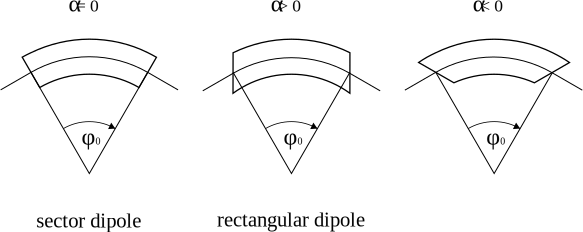
\includegraphics[width = \textwidth]{images/A-egde-focusing.pdf}
	\caption[Dipole magnets with different entrance and exit angles]{Dipole magnets with different entrance and exit angles (based on \cite{edge})}
	\label{fig:edge-angle-1}
\end{figure}
\noindent As shown in \autoref{fig:edge-angle-1} it possible to build dipole magnets with different entrance and exit angles~$\alpha$. Because of construction costs often rectangular magnets are used. The edge angle~$\alpha$ is defined in such a way that it is positive for a rectangular magnet. It influences the horizontal plane as well as the vertical plane and can be expressed due to a transfer matrix.

The effect on the horizontal motion is caused by changed path length within the dipole. As shown in \autoref{fig:edge-angle-2}, for a particle with a positive horizontal offset the path length is decreased by
\begin{figure}
	\centering
	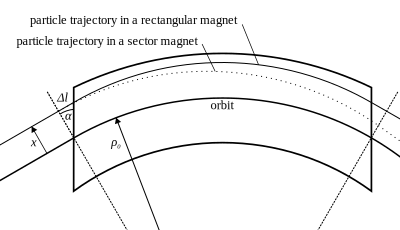
\includegraphics[width = 0.75\textwidth]{images/A-egde-focusing-horizontal.pdf}
	\caption{Edge focusing in the horizontal plane}
	\label{fig:edge-angle-2}
\end{figure}
\begin{align}
\Delta l = x \tan{\alpha} , 
\end{align}
while it is increased for a particle with negative horizontal offset. Therefore also the deflection angle $\varphi$ is changed:
\begin{align}
\Delta \varphi_{\textup{x}} = \frac{\Delta l}{\rho_{\textup{x0}}} = \frac{x \tan{\alpha}}{\rho_{\textup{x0}}} \quad \text{with} \quad \varphi_{\textup{x}} = \varphi_{0} - \Delta \varphi_{\textup{x}} 
\end{align}
As for small angles it is valid that
\begin{align}
\varphi_{\textup{x}} = \arctan{x'} \approx x', 
\end{align}
this can in thin lens approximation be written as a matrix:
\begin{equation}\begin{aligned}[b]
\textbf{R}_{\textup{edge,H}} = 
\begin{pmatrix} 
1 & 0 \\
\kap \tan{\alpha} & 1 \\
\end{pmatrix}
\end{aligned}\label{matrix-horizontaledgefocusing}\end{equation}
From \eqref{matrix-horizontaledgefocusing} we can see that the positive edge angle of a rectangular magnet leads to a defocussing in the horizontal plane. 

The vertical plane has a very similar matrix, even if it caused by a very different effect. The fringe fields of a dipole with an edge angle are not parallel to the orbit trajectory and have therefore also a horizontal component. This leads to the deflection angle 
\begin{figure}
	\centering
	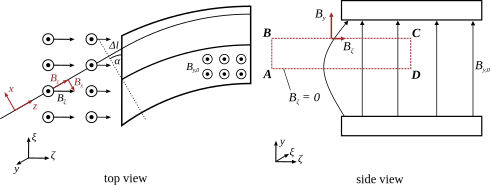
\includegraphics[width = \textwidth]{images/A-egde-focusing-vertical.pdf}
	\caption[Edge focusing in the vertical plane]{Edge focusing in the vertical plane (based on \cite{jankowiak})}
	\label{fig:edge-angle-3}
\end{figure}
\begin{align}
y' \approx \varphi_{\textup{y}} = \frac{q}{p} \int_{- \infty}^{+ \infty} B_{\textup{x}}(z) \du z 
\label{verticaldeflectionangle}\end{align}
in the vertical plane. As shown the in \autoref{fig:edge-angle-3} the horizontal field component can be written as
\begin{align}
B_{\textup{x}} = - \sin{\alpha} B_{\zeta}
\end{align}
We use the differential
\begin{align}
\du z = \frac{1}{\cos{\alpha}} \du \zeta
\end{align}
to substitute the integral of \eqref{verticaldeflectionangle}:
\begin{align}
\varphi_{\textup{y}} = - \frac{q \tan{\alpha}}{p} \int_{B}^{C} B_{\zeta}(\zeta) \du \zeta
\end{align}
As there are no magnetic monopoles we can use Gauss's law for magnetism
\begin{align}
0 = \oint \textbf{B} \du \textbf{r} = \int_{A}^{B} B_{\textup{y}} \du y + \int_{B}^{C} B_{\zeta} \du \zeta + \int_{C}^{D} B_{\textup{y}} \du y + \int_{D}^{A} B_{\zeta} \du \zeta,
\end{align}
where the first term is zero because of the field free region and the last term vanishes as $B_\zeta = 0$ in the symmetry plane. With
\begin{align}
\int_{B}^{C} B_{\zeta}(\zeta) \du \zeta = B_{\textup{y,0}} y
\end{align}
we obtain
\begin{align}
\varphi_{\textup{y}} = - \frac{q \tan{\alpha}}{p} B_{\textup{y,0}} y = - \kap \tan{\alpha}
\label{deflectionanglvertical2}\end{align}
for the vertical deflection angle. The matrix representation \eqref{deflectionanglvertical2} is given by:
\begin{equation}\begin{aligned}[b]
\textbf{R}_{\textup{edge,V}} = 
\begin{pmatrix} 
1 & 0 \\
-\kap \tan{\alpha} & 1 \\
\end{pmatrix}
\end{aligned}\label{matrix-verticaledgefocusing}\end{equation}


\chapter{Liouville's theorem} \label{appendixliouvillestheorem} 

To derive Liouville's equation it is more convenient to use the canonical coordinates $q_i$ and the conjugate momenta $p_i$. The phase space distribution $\rho(\textbf{q},\textbf{p},t)$ determines the number of particles $\rho(\textbf{q},\textbf{p},t) \du^s q \du^s p$ in the phase space volume $\du^s q  \du^s p$. The temporal change of particles in a region $G$ equals the flux through its surface $\partial G$ \cite{nolting6}. Therefore we obtain
\begin{equation}
\frac{\partial}{\partial t}\int_G \du^s q \du^s p \: \rho(\textbf{q},\textbf{p},t) = - \int_{\partial G} \du \textbf{S} \: \textbf{v} \cdot \rho(\textbf{q},\textbf{p},t) ,
\end{equation}
where \textbf{v} corresponds to the phase space velocity 
\begin{equation}
\textbf{v} = ( \dot{q}_1, ... , \dot{q}_s ,  \dot{p}_1, ... , \dot{p}_s) .
\end{equation}
According to Gauss's theorem the surface integral can be transformed to a volume integral, where the nabla is that of the \textit{2s}-dimensional phase space:
\begin{equation}
\int_G \du^s q \du^s p \left(\frac{\partial}{\partial t} \rho(\textbf{q},\textbf{p},t) + \nabla \textbf{v} \rho(\textbf{q},\textbf{p},t) \right) = 0
\label{liou1}\end{equation}
As we have the freedom to choose any region $G$, even the integrand has to disappear. Substituting of $\nabla = (\partial_{q_1},...,\partial_{q_s},\partial_{p_1},...,\partial_{p_s})$ into the integrand of (\ref{liou1}) yields
\begin{equation}
\frac{\partial \rho}{\partial t} + \sum_{i=1}^{s} \left(\frac{\partial \rho}{\partial q_i} \dot{q}_i+ \frac{\partial \rho}{\partial p_j} \dot{p}_i \right) + \rho \sum_{i=1}^{s}\left(\frac{\partial \dot{q}_i}{\partial q_i} +\frac{\partial \dot{p}_i}{\partial p_i} \right) = 0,
\end{equation}
where the second sum vanishes because of the Hamilton's equations $\dot{q} = \frac{\partial H}{\partial p}$ and $\dot{p} = -\frac{\partial H}{\partial q}$. This leads us to
\begin{equation}
\frac{\du \rho}{\du t} = \frac{\partial \rho}{\partial t} + \sum_{i=1}^{s} \left(\frac{\partial \rho}{\partial q_i} \dot{q}_i + \frac{\partial \rho}{\partial p_j} \dot{p}_i \right) = 0,
\end{equation}
which is known as Liouville's equation. It states that the phase space distribution along any path stays constant. Consequently also the volume of any area $G$, which moves through phase space, remains constant for all time\footnote{Identical particles with the same Hamiltonian can not cross in phase space. Therefore the inner and outer points of the region $G$ cannot to propagate through the surface area $\partial G$. Thus the number of phase space points within $G$ stays constant. As the phase space distribution is constant, the phase space volume of $G$ must be conserved.}. As we notice from the transfer matrices of \autoref{sectiontransfermatrix} the motion in the transversal planes decouples. Therefore the represented statements must already be true for the individual transversal dimensions. Besides that the Liouville's theorem does not make any statement about the shape of the area $G$, which can change over time.

The Liouville's theorem was tested for the time dependent Hamilton function:
\begin{equation}
H(q,p,t) = \frac{p^2}{2} + 2 t p  + \frac{\sin{q}}{2} - q \sqrt{t}
\end{equation}
The time evolution of the system is given by the Hamilton equations:
\begin{equation}\begin{aligned}[b]
\dot{q} &= \frac{\partial H}{\partial \textbf{p}} = p + 2 t\\
\dot{p} &= -\frac{\partial H}{\partial \textbf{q}} = - \frac{\cos{q}}{2} + \sqrt{t}
\end{aligned}\end{equation}
In \autoref{fig:liouvilleconstantvolume} the transformation of the area $G_0$ to $G_t$ after the time t is shown. In addition to that the trajectories of particles, which started within area $G_0$, are plotted. As one can see, the particles trajectories end within the area $G_t$ after the time t. Therefore the number of particles N within the area are constant. As the volume V remains the same the phase space density $p=\frac{N}{V}$ is, in accordance to Liouville's theorem, time independent.
\begin{figure}
	\centering
	\includegraphics[width = \textwidth]{images/A-liouville-theorem-constant-volume.pdf}
	\caption[Transformation of an arbitrary area in phase space.]{The ellipse $G_0$ is transformed to the the area $G_1$ after the time $t$. Additionally the individual trajectories for the red marked particles are shown.}
	\label{fig:liouvilleconstantvolume}
\end{figure}



\chapter{Detailed overview of all solutions}\label{chapter:allsolutions}

\def \nameofversion {Design}
\subsection*{The design lattice}
\pdfbookmark[section]{The design lattice}{The design lattice}
\begin{figure}[htbp!]
	\centering
	\includegraphics[width = \textwidth]{images/04-design-lattice.pdf}
	\caption{The design lattice of the Bessy II storage ring (1996).}
\end{figure}
\begin{table}[htbp!]
	\centering
	\footnotesize
	\caption{Quadrupole strengths of the design lattice.}
	\begin{tabular}{rrrrrr}
	\toprule
 $Q_{\textup{x}}$ / kHz &  $Q_{\textup{y}}$ / kHz &  $\beta_{\textup{x,max}}$ / m &  $\beta_{\textup{y,max}}$ / m &  $\overline{\beta}_{\textup{x,rel}}$ / m &  $\overline{\beta}_{\textup{y,rel}}$ / m \\
	\midrule
1061.71  &                  928.03 &                        17.6 &                         21.09    &                                      1.18  &                                    1.02 \\
\bottomrule
\end{tabular}
\\\begin{tabular}{lr}
\toprule
\textbf{Magnet} & \textbf{k} / m$^{-2}$\\
\midrule
Q1	& +2.45190 \\
Q2	& -1.89757\\
Q3D	& -2.02025\\
Q4D & +1.40816\\
Q3T & -2.46319\\
Q4T & +2.62081\\
Q5T & -2.60000\\
\bottomrule \\ \\
\end{tabular}


\end{table}
\newpage


\def \nameofversion {current}
\subsection*{The current standard lattice}
\pdfbookmark[section]{The current standard lattice}{The current standard lattice}
\begin{figure}[htbp!]
	\centering
	\includegraphics[width = \textwidth]{images/Overview-all-solutions/\nameofversion-comparison.pdf}
	\caption{The current standard lattice of the Bessy II storage ring (28.03.2017).}
\end{figure}
\begin{table}[htbp!]
	\centering
	\footnotesize
	\caption{Quadrupole strengths of the current standard lattice.}
	\begin{tabular}{rrrrrr}
	\toprule
 $Q_{\textup{x}}$ / kHz &  $Q_{\textup{y}}$ / kHz &  $\beta_{\textup{x,max}}$ / m &  $\beta_{\textup{y,max}}$ / m &  $\overline{\beta}_{\textup{x,rel}}$ / m &  $\overline{\beta}_{\textup{y,rel}}$ / m \\
	\midrule
 1060.54 &                  907.38 &                         26.14 &                         24.00 &                                     1.00 &                                     1.00 \\
\end{tabular}
\\\begin{tabular}{ll}
\toprule
\textbf{Magnet} & \textbf{k} / m$^{-2}$\\
\midrule
QIT6       & -1.09324443\\
Q1D        & +2.43992187\\
Q2D        & -1.85354137\\
Q3P1T1     & -2.53759435\\
Q3P1T6     & -2.68493846\\
Q3P1T8     & -2.44627319\\
Q3P2T1     & -2.44026692\\
Q3P2T6     & -2.33722602\\
Q3P2T8     & -2.53960920\\
Q3D1       & -2.02056340\\
Q3D2       & -2.12545914\\
Q3D3       & -2.12560233\\
Q3D4       & -2.13235047\\
Q3D5       & -2.11955588\\
Q3D6       & -2.10963250\\
Q3D7       & -2.11735207\\
Q3D8       & -2.13655479\\
\bottomrule \\ \\
\end{tabular}
\begin{tabular}{ll}
\toprule
\textbf{Magnet} & \textbf{k} / m$^{-2}$\\
\midrule
Q3T2       & -2.45516822\\
Q3T3       & -2.42796219\\
Q3T4       & -2.43958732\\
Q3T5       & -2.44973680\\
Q3T7       & -2.43215097\\
Q4P1T1     & +2.61530699\\
Q4P1T6     & +2.24854535\\
Q4P1T8     & +2.58252211\\
Q4P2T1     & +2.58203605\\
Q4P2T6     & +2.56031750\\
Q4P2T8     & +2.62213165\\
Q4D1       & +1.40197290\\
Q4D2       & +1.47885355\\
Q4D3       & +1.48649031\\
Q4D4       & +1.49263679\\
Q4D5       & +1.47760503\\
Q4D6       & +1.48292220\\
Q4D7       & +1.47659449\\
Q4D8       & +1.49275949\\
\bottomrule
\end{tabular}
\begin{tabular}{ll}
\toprule
\textbf{Magnet} & \textbf{k} / m$^{-2}$\\
\midrule
Q4T2       & +2.57898949\\
Q4T3       & +2.57796719\\
Q4T4       & +2.58157782\\
Q4T5       & +2.58022594\\
Q4T7       & +2.58000776\\
Q5P1T1     & -2.42116424\\
Q5P1T6     & -1.02671552\\
Q5P1T8     & -2.59460394\\
Q5P2T1     & -2.60077137\\
Q5P2T6     & -2.45473858\\
Q5P2T8     & -2.41402770\\
Q5T2       & -2.58798946\\
Q5T3       & -2.62810235\\
Q5T4       & -2.59997779\\
Q5T5       & -2.59005859\\
Q5T7       & -2.60805533\\
\bottomrule \\ \\ \\
\end{tabular}

	\label{tab:standard2017quadsrengths}
\end{table}
\newpage


\def \nameofversion {V1}
\subsection*{\nameofversion}
\pdfbookmark[section]{\nameofversion}{\nameofversion}
\begin{figure}[htbp!]
	\centering
	\includegraphics[width = \textwidth]{images/Overview-all-solutions/\nameofversion-comparison.pdf}
	\caption{Comparison of the \nameofversion -lattice with the current lattice.}
\end{figure}
\begin{table}[htbp!]
	\centering
	\footnotesize
	\caption{Fit output \nameofversion.}
	\input{tables/\nameofversion.tex}
\end{table}
\newpage

\def \nameofversion {V2}
\subsection*{\nameofversion}
\pdfbookmark[section]{\nameofversion}{\nameofversion}
\begin{figure}[htbp!]
	\centering
	\includegraphics[width = \textwidth]{images/Overview-all-solutions/\nameofversion-comparison.pdf}
	\caption{Comparison of the \nameofversion -lattice with the current lattice.}
\end{figure}
\begin{table}[htbp!]
	\centering
	\footnotesize
	\caption{Fit output \nameofversion.}
	\input{tables/\nameofversion.tex}
\end{table}
\newpage

\def \nameofversion {V3}
\subsection*{\nameofversion}
\pdfbookmark[section]{\nameofversion}{\nameofversion}
\begin{figure}[htbp!]
	\centering
	\includegraphics[width = \textwidth]{images/Overview-all-solutions/\nameofversion-comparison.pdf}
	\caption{Comparison of the \nameofversion -lattice with the current lattice.}
\end{figure}
\begin{table}[htbp!]
	\centering
	\footnotesize
	\caption{Fit output \nameofversion.}
	\input{tables/\nameofversion.tex}
\end{table}
\newpage



\def \nameofversion {V4}
\subsection*{\nameofversion}
\pdfbookmark[section]{\nameofversion}{\nameofversion}
\begin{figure}[htbp!]
	\centering
	\includegraphics[width = \textwidth]{images/Overview-all-solutions/\nameofversion-comparison.pdf}
	\caption{Comparison of the \nameofversion -lattice with the current lattice.}
\end{figure}
\begin{table}[htbp!]
	\centering
	\footnotesize
	\caption{Fit output \nameofversion.}
	\input{tables/\nameofversion.tex}
\end{table}
\newpage




\def \nameofversion {V5}
\subsection*{\nameofversion}
\pdfbookmark[section]{\nameofversion}{\nameofversion}
\begin{figure}[htbp!]
	\centering
	\includegraphics[width = \textwidth]{images/Overview-all-solutions/\nameofversion-comparison.pdf}
	\caption{Comparison of the \nameofversion -lattice with the current lattice.}
\end{figure}
\begin{table}[htbp!]
	\centering
	\footnotesize
	\caption{Fit output \nameofversion.}
	\input{tables/\nameofversion.tex}
\end{table}
\newpage



\def \nameofversion {Vall}
\subsection*{\nameofversion}
\pdfbookmark[section]{\nameofversion}{\nameofversion}
\begin{figure}[htbp!]
	\centering
	\includegraphics[width = \textwidth]{images/Overview-all-solutions/\nameofversion-comparison.pdf}
	\caption{Comparison of the \nameofversion -lattice with the current lattice.}
\end{figure}
\begin{table}[htbp!]
	\centering
	\footnotesize
	\caption{Fit output \nameofversion.}
	\input{tables/\nameofversion.tex}
\end{table}
\newpage



\def \nameofversion {V2Q3T}
\subsection*{\nameofversion}
\pdfbookmark[section]{\nameofversion}{\nameofversion}
\begin{figure}[htbp!]
	\centering
	\includegraphics[width = \textwidth]{images/Overview-all-solutions/\nameofversion-comparison.pdf}
	\caption{Comparison of the \nameofversion -lattice with the current lattice.}
\end{figure}
\begin{table}[htbp!]
	\centering
	\footnotesize
	\caption{Fit output \nameofversion.}
	\input{tables/\nameofversion.tex}
\end{table}
\newpage


\def \nameofversion {V2Q4T}
\subsection*{\nameofversion}
\pdfbookmark[section]{\nameofversion}{\nameofversion}
\begin{figure}[htbp!]
	\centering
	\includegraphics[width = \textwidth]{images/Overview-all-solutions/\nameofversion-comparison.pdf}
	\caption{Comparison of the \nameofversion -lattice with the current lattice.}
\end{figure}
\begin{table}[htbp!]
	\centering
	\footnotesize
	\caption{Fit output \nameofversion.}
	\input{tables/\nameofversion.tex}
\end{table}
\newpage


\def \nameofversion {V2Q5}
\subsection*{\nameofversion}
\pdfbookmark[section]{\nameofversion}{\nameofversion}
\begin{figure}[htbp!]
	\centering
	\includegraphics[width = \textwidth]{images/Overview-all-solutions/\nameofversion-comparison.pdf}
	\caption{Comparison of the \nameofversion -lattice with the current lattice.}
\end{figure}
\begin{table}[htbp!]
	\centering
	\footnotesize
	\caption{Fit output \nameofversion.}
	\input{tables/\nameofversion.tex}
\end{table}
\newpage

\def \nameofversion {VOF}
\subsection*{\nameofversion}
\pdfbookmark[section]{\nameofversion}{\nameofversion}
\begin{figure}[htbp!]
	\centering
	\includegraphics[width = \textwidth]{images/Overview-all-solutions/\nameofversion-comparison.pdf}
	\caption{Comparison of the \nameofversion -lattice with the current lattice.}
\end{figure}
\begin{table}[htbp!]
	\centering
	\footnotesize
	\caption{Fit output \nameofversion.}
	\input{tables/\nameofversion.tex}
\end{table}
\newpage


\subsection*{LOCO measurements}
\pdfbookmark[section]{LOCO measurements of the new optics}{LOCO measurements of the new optics}

\subsection*{V1: LOCO vs SIM}
\begin{figure}[htbp!]
	\centering
	\includegraphics[width = \textwidth]{images/Overview-all-solutions/A-V1_LOCO_vs_SIM.pdf}
	\caption{Comparison of V1 LOCO (solid) with V1 SIM (dashed).}
	\label{fig:V1-LOCO-vs-SIM}
\end{figure}

\subsection*{V2: LOCO vs SIM}
\begin{figure}[htbp!]
	\centering
	\includegraphics[width = \textwidth]{images/Overview-all-solutions/A-V2_LOCO_vs_SIM.pdf}
	\caption{Comparison of V2 LOCO (solid) with V2 SIM (dashed).}
	\label{fig:V2-LOCO-vs-SIM}
\end{figure}


\newpage
\subsection*{V4 LOCO vs SIM (MAY)}
\begin{figure}[htbp!]
	\centering
	\includegraphics[width = \textwidth]{images/05-V4_LOCO_vs_SIM.pdf}
	\caption{Comparison of V4 LOCO (solid) with V4 SIM (dashed) of May.}
\end{figure}

\subsection*{V4 LOCO vs SIM LOCO (AUG)}
\begin{figure}[htbp!]
	\centering
	\includegraphics[width = \textwidth]{images/Overview-all-solutions/A-V4_LOCO_vs_SIM_AUG.pdf}
	\caption{Comparison of V4 LOCO (solid) with V4 SIM (dashed) of August.}
	\label{fig:V4-LOCO-vs-SIM_AUG}
\end{figure}


\newpage
\subsection*{V4 LOCO August vs Stanard LOCO}
\begin{figure}[htbp!]
	\centering
	\includegraphics[width = \textwidth]{images/05-V4_vs_standard_loco.pdf}
	\caption{The loco measured V4 optics (solid) in comparison to the standard optics (dashed).}
\end{figure}


\subsection*{Standard: August vs March}
\begin{figure}[htbp!]
	\centering
	\includegraphics[width = \textwidth]{images/Overview-all-solutions/A-comparison-standard-optics-august-vs-march.pdf}
	\caption{Comparison of the LOCO measured standard optics from 04.08.2017 with 28.03.2017.}
	\label{fig:standard-comparison}
\end{figure}





%----------------------------------------------------------------------------------------
%	BIBLIOGRAPHY
%----------------------------------------------------------------------------------------
\renewcommand*{\newunitpunct}{\addcomma\space} % komma statt punkt
\printbibliography[heading=bibintoc]


%----------------------------------------------------------------------------------------
%	DECLARATION PAGE
%----------------------------------------------------------------------------------------
\begin{declaration}
	\addchaptertocentry{\authorshipname} % Add the declaration to the table of contents

	\noindent I, \authorname, declare that this thesis and the work presented in it are my own. I confirm that where I have quoted from the work of others, the source is always given.
	%\noindent I, \authorname, declare that this thesis titled, \enquote{\ttitle} and the work presented in it are my own. I confirm that:
	%
	%\begin{itemize} 
	%\item This work was done wholly or mainly while in candidature for a research degree at this University.
	%\item Where any part of this thesis has previously been submitted for a degree or any other qualification at this University or any other institution, this has been clearly stated.
	%\item Where I have consulted the published work of others, this is always clearly attributed.
	%\item Where I have quoted from the work of others, the source is always given. With the exception of such quotations, this thesis is entirely my own work.
	%\item I have acknowledged all main sources of help.
	%\item Where the thesis is based on work done by myself jointly with others, I have made clear exactly what was done by others and what I have contributed myself.\\
	%\end{itemize}
	% 
	\vspace{3cm}

	\noindent Signature:\\
	\rule[0.5em]{25em}{0.5pt} % This prints a line for the signature

	\noindent Place, Date: \hspace{3cm}Berlin, \today\\
	\rule[0.5em]{25em}{0.5pt} % This prints a line to write the date
\end{declaration}

\cleardoublepage

\end{document}